% ============================================================
%  Math/Physics 89 — Personal Notes
%  Boas: Mathematical Methods in the Physical Sciences
%  Chapters: 1–8, 10, 12–14 (§1–7)
% ============================================================

\documentclass[11pt, letterpaper]{article}

% ── Packages ────────────────────────────────────────────────
\usepackage[margin=1in]{geometry}
\usepackage{amsmath, amssymb, amsthm}
\usepackage{mathtools}
\usepackage{physics}
\usepackage{bm}
\usepackage{esint}
\usepackage{enumerate}
\usepackage{hyperref}
\usepackage{tcolorbox}
\usepackage{booktabs}
\usepackage{fancyhdr}
\usepackage{xcolor}
\usepackage{graphicx}

% ── tcolorbox ───────────────────────────────────────────────

\tcbuselibrary{theorems, skins, breakable}

\definecolor{defblue}{RGB}{30, 90, 160}
\definecolor{thmgreen}{RGB}{20, 130, 80}
\definecolor{exorange}{RGB}{200, 100, 20}

\newtcbtheorem[number within=section]{definition}{Definition}%
  {colback=defblue!8, colframe=defblue!60, fonttitle=\bfseries, breakable}{def}

\newtcbtheorem[number within=section]{theorem}{Theorem}%
  {colback=thmgreen!8, colframe=thmgreen!60, fonttitle=\bfseries, breakable}{thm}

\newtcbtheorem[number within=section]{example}{Example}%
  {colback=exorange!8, colframe=exorange!60, fonttitle=\bfseries, breakable}{ex}

% ── AMS environments ────────────────────────────────────────
\theoremstyle{plain}
\newtheorem{lemma}{Lemma}[section]
\newtheorem{corollary}{Corollary}[section]
\newtheorem{proposition}{Proposition}[section]

\newenvironment{remark}{\smallskip\noindent\textit{Remark.}}{\smallskip}

% ── Macros ──────────────────────────────────────────────────
\newcommand{\R}{\mathbb{R}}
\newcommand{\C}{\mathbb{C}}
\newcommand{\N}{\mathbb{N}}
\newcommand{\Z}{\mathbb{Z}}
\newcommand{\vv}[1]{\bm{#1}}
\renewcommand{\Re}{\operatorname{Re}}
\renewcommand{\Im}{\operatorname{Im}}
\renewcommand{\Res}{\operatorname{Res}}
\DeclareMathOperator{\Arg}{Arg}

% ── Header / Footer ─────────────────────────────────────────
\pagestyle{fancy}
\fancyhf{}
\lhead{\small Physics 89}
\chead{\small \leftmark}
\rhead{\small Boas}
\cfoot{\small \thepage}
\renewcommand{\headrulewidth}{0.4pt}

% ── Title ───────────────────────────────────────────────────
\title{%
  \textbf{Textbook — Notes}\\[4pt]
  \large Boas: \textit{Mathematical Methods in the Physical Sciences}
}
\author{}
\date{\today}


% ============================================================
\begin{document}
% ============================================================


\maketitle
\tableofcontents
\newpage


% ============================================================
\section{Infinite Series, Power Series}        % Ch. 1
% ============================================================

\subsection{Series Definitions}

A \textbf{sequence} is an ordered list $\{a_n\}_{n=1}^\infty$. A \textbf{series}
is the sum of a sequence:
\[
    S = \sum_{n=1}^{\infty} a_n = a_1 + a_2 + a_3 + \cdots
\]
The \textbf{partial sum} is $S_N = \sum_{n=1}^N a_n$.
The series converges if $\lim_{N\to\infty} S_N = S$ exists and is finite;
otherwise it diverges.

\subsubsection*{Geometric Series}
\[
    \sum_{n=0}^{\infty} ar^n = \frac{a}{1-r}, \qquad |r| < 1
\]
Diverges for $|r| \geq 1$. This is the most useful series to recognize.

\subsubsection*{Harmonic and $p$-Series}
\[
    \sum_{n=1}^{\infty} \frac{1}{n^p} \begin{cases}
        \text{converges} & p > 1 \\
        \text{diverges}  & p \leq 1
    \end{cases}
\]
The harmonic series $\sum 1/n$ ($p=1$) diverges.


\subsection{Convergence and Divergence}

\begin{definition}{Absolute and Conditional Convergence}{absconv}
    A series $\sum a_n$ \emph{converges absolutely} if $\sum |a_n|$ converges.
    It \emph{converges conditionally} if $\sum a_n$ converges but
    $\sum |a_n|$ diverges. Absolute convergence implies convergence.
\end{definition}

\subsubsection*{Necessary Condition for Convergence}
If $\sum a_n$ converges, then $\lim_{n\to\infty} a_n = 0$.
The converse is \emph{false} (e.g.\ harmonic series).

\subsubsection*{Alternating Series}
An alternating series $\sum (-1)^n a_n$ with $a_n > 0$ converges if:
\begin{enumerate}[(i)]
    \item $a_n$ is eventually decreasing: $a_{n+1} \leq a_n$
    \item $\lim_{n\to\infty} a_n = 0$
\end{enumerate}
The error from truncating at $N$ terms is bounded by $|a_{N+1}|$.


\subsection{Convergence Tests}

\begin{center}
\begin{tabular}{lll}
    \toprule
    Test & Condition & Conclusion \\
    \midrule
    \textbf{Divergence} & $\lim a_n \neq 0$ & diverges \\[4pt]
    \textbf{Ratio} & $L = \lim\left|\dfrac{a_{n+1}}{a_n}\right|$ &
        $L<1$: conv.; $L>1$: div.; $L=1$: ? \\[8pt]
    \textbf{Root} & $L = \lim |a_n|^{1/n}$ &
        $L<1$: conv.; $L>1$: div.; $L=1$: ? \\[4pt]
    \textbf{Integral} & $\int_1^\infty f(x)\,dx$ converges & $\sum f(n)$ converges \\[4pt]
    \textbf{Comparison} & $0 \leq a_n \leq b_n$ &
        $\sum b_n$ conv. $\Rightarrow$ $\sum a_n$ conv. \\[4pt]
    \textbf{Limit Comp.} & $\lim \frac{a_n}{b_n} = c > 0$ &
        $\sum a_n$ and $\sum b_n$ same behavior \\
    \bottomrule
\end{tabular}
\end{center}

\begin{remark}
    The ratio test is best for factorials and exponentials.
    The root test is best for terms of the form $(f(n))^n$.
    The integral test works well for $1/n^p$, $1/(n\ln n)$, etc.
\end{remark}


\subsection{Power Series}

A \textbf{power series} centered at $a$ is:
\[
    \sum_{n=0}^{\infty} c_n(x-a)^n = c_0 + c_1(x-a) + c_2(x-a)^2 + \cdots
\]

\subsubsection*{Radius of Convergence}
By the ratio test, the series converges for $|x - a| < R$ where:
\[
    R = \lim_{n\to\infty}\left|\frac{c_n}{c_{n+1}}\right|
    \quad \text{or} \quad
    \frac{1}{R} = \limsup_{n\to\infty}|c_n|^{1/n}
\]
The series diverges for $|x-a| > R$. At $|x-a| = R$ check separately.
$R = 0$: converges only at $x=a$. $R = \infty$: converges everywhere.

\subsubsection*{Operations on Power Series}
Within the radius of convergence, power series can be:
\begin{itemize}
    \item Added, subtracted, and multiplied term by term
    \item \textbf{Differentiated:}
          $\dv{}{x}\sum c_n(x-a)^n = \sum n\,c_n(x-a)^{n-1}$
    \item \textbf{Integrated:}
          $\int\sum c_n(x-a)^n\,dx = \sum \dfrac{c_n}{n+1}(x-a)^{n+1} + C$
\end{itemize}
Both operations preserve the radius of convergence.


\subsection{Taylor and Maclaurin Series}

If $f$ is infinitely differentiable at $x = a$, its \textbf{Taylor series} is:
\[
    f(x) = \sum_{n=0}^{\infty} \frac{f^{(n)}(a)}{n!}(x-a)^n
\]
A \textbf{Maclaurin series} is a Taylor series centered at $a = 0$.

\subsubsection*{Standard Maclaurin Series}
\[
    e^x = \sum_{n=0}^{\infty}\frac{x^n}{n!}, \qquad R = \infty
\]
\[
    \sin x = \sum_{n=0}^{\infty}\frac{(-1)^n x^{2n+1}}{(2n+1)!}, \qquad R = \infty
\]
\[
    \cos x = \sum_{n=0}^{\infty}\frac{(-1)^n x^{2n}}{(2n)!}, \qquad R = \infty
\]
\[
    \ln(1+x) = \sum_{n=1}^{\infty}\frac{(-1)^{n+1}x^n}{n}
    = x - \frac{x^2}{2} + \frac{x^3}{3} - \cdots, \qquad R = 1
\]
\[
    \frac{1}{1-x} = \sum_{n=0}^{\infty} x^n, \qquad R = 1
\]

\subsubsection*{Taylor Remainder}
The error from truncating at degree $N$ is:
\[
    R_N(x) = \frac{f^{(N+1)}(\xi)}{(N+1)!}(x-a)^{N+1}
\]
for some $\xi$ between $a$ and $x$ (Lagrange form).


\subsection{Binomial Series}

For any real exponent $p$:
\[
    (1+x)^p = \sum_{n=0}^{\infty}\binom{p}{n}x^n, \qquad |x| < 1
\]
where the \textbf{generalized binomial coefficient} is:
\[
    \binom{p}{n} = \frac{p(p-1)(p-2)\cdots(p-n+1)}{n!}, \qquad \binom{p}{0} = 1
\]

\subsubsection*{Common Special Cases}
\[
    \frac{1}{1+x} = 1 - x + x^2 - x^3 + \cdots \qquad (p = -1)
\]
\[
    \frac{1}{\sqrt{1+x}} = 1 - \frac{x}{2} + \frac{3x^2}{8} - \cdots \qquad (p = -\tfrac{1}{2})
\]
\[
    \sqrt{1+x} = 1 + \frac{x}{2} - \frac{x^2}{8} + \cdots \qquad (p = \tfrac{1}{2})
\]

\begin{remark}
    For $p$ a non-negative integer, the binomial series terminates after
    $p+1$ terms and is just the usual binomial theorem, valid for all $x$.
    For all other $p$, the series is infinite with radius of convergence $R=1$.
\end{remark}


\newpage
% ============================================================
\section{Complex Numbers}                      % Ch. 2
% ============================================================

\subsection{Complex Algebra}

A \textbf{complex number} is $z = x + iy$ where $x,y\in\mathbb{R}$ and
$i^2 = -1$. We call $x = \Re(z)$ the real part and $y = \Im(z)$ the
imaginary part.

\subsubsection*{Basic Operations}
For $z_1 = x_1 + iy_1$ and $z_2 = x_2 + iy_2$:
\[
    z_1 \pm z_2 = (x_1 \pm x_2) + i(y_1 \pm y_2)
\]
\[
    z_1 z_2 = (x_1 x_2 - y_1 y_2) + i(x_1 y_2 + x_2 y_1)
\]
\[
    \frac{z_1}{z_2} = \frac{z_1\bar{z}_2}{|z_2|^2}
    = \frac{(x_1 x_2 + y_1 y_2) + i(x_2 y_1 - x_1 y_2)}{x_2^2 + y_2^2}
\]

\subsubsection*{Complex Conjugate}
$\bar{z} = x - iy$. Key identities:
\[
    z\bar{z} = x^2 + y^2 = |z|^2, \qquad
    \Re(z) = \frac{z+\bar{z}}{2}, \qquad
    \Im(z) = \frac{z-\bar{z}}{2i}
\]
\[
    \overline{z_1 + z_2} = \bar{z}_1 + \bar{z}_2, \qquad
    \overline{z_1 z_2} = \bar{z}_1\bar{z}_2
\]

\subsubsection*{Modulus}
\[
    |z| = \sqrt{x^2 + y^2}, \qquad
    |z_1 z_2| = |z_1||z_2|, \qquad
    \left|\frac{z_1}{z_2}\right| = \frac{|z_1|}{|z_2|}
\]
\textbf{Triangle inequality:} $|z_1 + z_2| \leq |z_1| + |z_2|$.


\subsection{Polar Form and Euler's Formula}

Every complex number can be written in polar form:
\[
    z = r e^{i\theta} = r(\cos\theta + i\sin\theta)
\]
where $r = |z| \geq 0$ and $\theta = \arg(z) = \arctan(y/x)$.

\begin{definition}{Principal Value of Argument}{arg}
    The \emph{principal argument} $\Arg(z)\in(-\pi,\pi]$ is the unique
    angle in that range. The general argument is $\arg(z) = \Arg(z) + 2\pi k$
    for $k\in\mathbb{Z}$.
\end{definition}

\subsubsection*{Euler's Formula}
\[
    e^{i\theta} = \cos\theta + i\sin\theta
\]
Special cases:
\[
    e^{i\pi} + 1 = 0, \qquad e^{i\pi/2} = i, \qquad e^{-i\theta} = \cos\theta - i\sin\theta
\]
Expressing trig functions in terms of exponentials:
\[
    \cos\theta = \frac{e^{i\theta} + e^{-i\theta}}{2}, \qquad
    \sin\theta = \frac{e^{i\theta} - e^{-i\theta}}{2i}
\]

\subsubsection*{Multiplication in Polar Form}
\[
    z_1 z_2 = r_1 r_2\, e^{i(\theta_1+\theta_2)}, \qquad
    \frac{z_1}{z_2} = \frac{r_1}{r_2}\,e^{i(\theta_1 - \theta_2)}
\]
Multiplication rotates and scales; division does the reverse.


\subsection{Hyperbolic Functions}

Defined in analogy with trig functions via exponentials:
\[
    \cosh z = \frac{e^z + e^{-z}}{2}, \qquad
    \sinh z = \frac{e^z - e^{-z}}{2}, \qquad
    \tanh z = \frac{\sinh z}{\cosh z}
\]

\subsubsection*{Key Identities}
\[
    \cosh^2 z - \sinh^2 z = 1
\]
\[
    \cosh(iz) = \cos z, \qquad \sinh(iz) = i\sin z
\]
\[
    \cos(iz) = \cosh z, \qquad \sin(iz) = i\sinh z
\]

\subsubsection*{Complex Trig and Hyperbolic Functions}
For $z = x + iy$:
\[
    \sin z = \sin x\cosh y + i\cos x\sinh y
\]
\[
    \cos z = \cos x\cosh y - i\sin x\sinh y
\]

\begin{remark}
    Unlike real trig functions, $|\sin z|$ and $|\cos z|$ are not bounded
    by 1 for complex $z$ — they can be arbitrarily large.
\end{remark}


\subsection{Powers and Roots}

\subsubsection*{De Moivre's Theorem}
\[
    z^n = r^n e^{in\theta} = r^n(\cos n\theta + i\sin n\theta)
\]
Useful for deriving multiple-angle formulas, e.g.\
$\cos 3\theta = \Re[(\cos\theta + i\sin\theta)^3]$.

\subsubsection*{$n$-th Roots}
The equation $w^n = z$ has exactly $n$ solutions:
\[
    w_k = r^{1/n}\exp\!\left[i\left(\frac{\theta + 2\pi k}{n}\right)\right],
    \qquad k = 0, 1, \ldots, n-1
\]
The $n$ roots are equally spaced on a circle of radius $r^{1/n}$.

\begin{example}{Cube roots of unity}{cuberoots}
    The solutions to $w^3 = 1$ (i.e.\ $r=1$, $\theta=0$) are:
    \[
        w_k = e^{2\pi ik/3}, \quad k = 0,1,2
        \implies 1,\quad -\tfrac{1}{2}+i\tfrac{\sqrt{3}}{2},\quad
        -\tfrac{1}{2}-i\tfrac{\sqrt{3}}{2}
    \]
    They form an equilateral triangle inscribed in the unit circle.
\end{example}


\subsection{The Complex Plane; Sets}

The complex plane (\textbf{Argand diagram}) represents $z = x+iy$
as the point $(x,y)$. Key sets:
\begin{itemize}
    \item \textbf{Disk:} $|z - z_0| < r$ — open disk of radius $r$ centered at $z_0$
    \item \textbf{Circle:} $|z - z_0| = r$
    \item \textbf{Annulus:} $r_1 < |z - z_0| < r_2$
    \item \textbf{Half-plane:} $\Re(z) > 0$ or $\Im(z) > 0$, etc.
\end{itemize}

\begin{definition}{Simply Connected}{simplycon}
    A region $D$ is \emph{simply connected} if every closed curve in $D$
    can be continuously shrunk to a point without leaving $D$ —
    i.e.\ $D$ has no holes.
\end{definition}


\subsection{Complex Functions}

A complex function $f: \mathbb{C}\to\mathbb{C}$ can be written as:
\[
    f(z) = u(x,y) + iv(x,y)
\]
where $u$ and $v$ are real-valued functions of two real variables.

\subsubsection*{Examples}
\[
    f(z) = z^2 = (x^2 - y^2) + i(2xy)
    \implies u = x^2 - y^2,\quad v = 2xy
\]
\[
    e^z = e^x\cos y + ie^x\sin y
    \implies u = e^x\cos y,\quad v = e^x\sin y
\]

\subsubsection*{Complex Logarithm}
\[
    \ln z = \ln|z| + i\arg(z) = \ln r + i(\theta + 2\pi k), \quad k\in\mathbb{Z}
\]
Multi-valued due to the $2\pi k$ ambiguity. The \textbf{principal value}
uses $\theta = \Arg(z)\in(-\pi,\pi]$:
\[
    \text{Log}\,z = \ln r + i\,\Arg(z)
\]

\subsubsection*{Complex Powers}
\[
    z^c = e^{c\ln z}
\]
Multi-valued in general since $\ln z$ is multi-valued.


\subsection{Cauchy--Riemann Equations}

\begin{theorem}{Cauchy--Riemann Equations}{CR}
    $f(z) = u + iv$ is analytic at $z_0$ if and only if the partial
    derivatives of $u$ and $v$ exist, are continuous, and satisfy:
    \[
        \pdv{u}{x} = \pdv{v}{y}, \qquad \pdv{u}{y} = -\pdv{v}{x}
    \]
    at $z_0$. The derivative is then:
    \[
        f'(z) = \pdv{u}{x} + i\pdv{v}{x} = \pdv{v}{y} - i\pdv{u}{y}
    \]
\end{theorem}

\subsubsection*{Harmonic Functions}
If $f = u + iv$ is analytic, both $u$ and $v$ satisfy Laplace's equation:
\[
    \nabla^2 u = \pdv[2]{u}{x} + \pdv[2]{u}{y} = 0, \qquad
    \nabla^2 v = \pdv[2]{v}{x} + \pdv[2]{v}{y} = 0
\]
$u$ and $v$ are called \emph{harmonic conjugates}.
Given $u$, find $v$ by integrating the C--R equations.

\begin{example}{Checking analyticity}{CR-ex}
    Is $f(z) = \bar{z} = x - iy$ analytic? Here $u = x$, $v = -y$.
    Check C--R: $\pdv{u}{x} = 1$ but $\pdv{v}{y} = -1$. Since $1\neq -1$,
    the C--R equations fail everywhere and $f(z) = \bar{z}$ is
    \emph{nowhere analytic}.
\end{example}

\begin{remark}
    In polar coordinates $(r,\theta)$, the C--R equations become:
    \[
        \pdv{u}{r} = \frac{1}{r}\pdv{v}{\theta}, \qquad
        \frac{1}{r}\pdv{u}{\theta} = -\pdv{v}{r}
    \]
\end{remark}

\newpage
% ============================================================
\section{Linear Algebra}                       % Ch. 3
% ============================================================

\subsection{Matrices and Determinants}

An $m\times n$ matrix $A$ has $m$ rows and $n$ columns. Entry in row $i$,
column $j$ is $A_{ij}$ or $a_{ij}$.

\subsubsection*{Matrix Operations}
\[
    (AB)_{ij} = \sum_k A_{ik}B_{kj}, \qquad
    (A^T)_{ij} = A_{ji}, \qquad
    (AB)^T = B^T A^T
\]
Matrix multiplication is associative and distributive but \emph{not}
generally commutative: $AB \neq BA$.

\subsubsection*{Determinant}
For a $2\times 2$ matrix:
\[
    \det\begin{pmatrix} a & b \\ c & d \end{pmatrix} = ad - bc
\]
For larger matrices, expand along any row or column (cofactor expansion).
Key properties:
\begin{itemize}
    \item $\det(AB) = \det(A)\det(B)$
    \item $\det(A^T) = \det(A)$
    \item $\det(A^{-1}) = 1/\det(A)$
    \item Swapping two rows (columns) flips the sign of $\det$
    \item A row of zeros or two identical rows $\Rightarrow$ $\det = 0$
\end{itemize}

\subsubsection*{Inverse}
$A^{-1}$ exists if and only if $\det(A) \neq 0$ ($A$ is \emph{nonsingular}).
\[
    AA^{-1} = A^{-1}A = I, \qquad
    (AB)^{-1} = B^{-1}A^{-1}
\]
For $2\times 2$:
\[
    \begin{pmatrix} a & b \\ c & d \end{pmatrix}^{-1}
    = \frac{1}{ad-bc}\begin{pmatrix} d & -b \\ -c & a \end{pmatrix}
\]

\subsubsection*{Trace}
\[
    \text{tr}(A) = \sum_i A_{ii}, \qquad
    \text{tr}(AB) = \text{tr}(BA)
\]


\subsection{Linear Systems; Row Reduction}

A system $A\vv{x} = \vv{b}$ has:
\begin{itemize}
    \item A unique solution if $\det(A) \neq 0$
    \item No solution or infinitely many solutions if $\det(A) = 0$
\end{itemize}

\subsubsection*{Gaussian Elimination}
Reduce the augmented matrix $[A\,|\,\vv{b}]$ to row echelon form using:
\begin{enumerate}[(i)]
    \item Swap two rows
    \item Multiply a row by a nonzero scalar
    \item Add a multiple of one row to another
\end{enumerate}
\textbf{Gauss--Jordan elimination} continues to \emph{reduced} row echelon
form (RREF), directly yielding the solution.

\subsubsection*{Rank}
The \textbf{rank} of $A$ is the number of nonzero rows in its row echelon
form $=$ the number of linearly independent rows (or columns).
\[
    \text{rank}(A) + \text{nullity}(A) = n \quad \text{(columns of }A\text{)}
\]


\subsection{Linear Dependencies}

A set of vectors $\{\vv{v}_1, \ldots, \vv{v}_n\}$ is \textbf{linearly dependent}
if there exist scalars $c_1,\ldots,c_n$, not all zero, such that:
\[
    c_1\vv{v}_1 + c_2\vv{v}_2 + \cdots + c_n\vv{v}_n = \vv{0}
\]
Otherwise the set is \textbf{linearly independent}.

\subsubsection*{Testing for Dependence}
Form the matrix with $\vv{v}_i$ as columns and row reduce.
The vectors are linearly dependent if and only if $\det = 0$
(for a square matrix), or equivalently if rank $< n$.

\subsubsection*{Wronskian (for functions)}
For functions $f_1,\ldots,f_n$, the Wronskian is:
\[
    W(x) = \begin{vmatrix}
        f_1 & f_2 & \cdots & f_n \\
        f_1' & f_2' & \cdots & f_n' \\
        \vdots & & & \vdots \\
        f_1^{(n-1)} & f_2^{(n-1)} & \cdots & f_n^{(n-1)}
    \end{vmatrix}
\]
If $W(x) \neq 0$ for some $x$, the functions are linearly independent.


\subsection{Vector Spaces and Subspaces}

\begin{definition}{Vector Space}{vecspace}
    A \emph{vector space} over $\mathbb{R}$ is a set $V$ with operations
    of addition and scalar multiplication satisfying the usual axioms
    (commutativity, associativity, distributivity, identity, inverses).
\end{definition}

A \textbf{subspace} $W \subseteq V$ must satisfy:
\begin{enumerate}[(i)]
    \item $\vv{0} \in W$
    \item $\vv{u}, \vv{v} \in W \Rightarrow \vv{u}+\vv{v} \in W$ (closed under addition)
    \item $\vv{v}\in W,\, c\in\mathbb{R} \Rightarrow c\vv{v}\in W$ (closed under scalar mult.)
\end{enumerate}

\subsubsection*{Basis and Dimension}
A \textbf{basis} is a linearly independent spanning set.
The \textbf{dimension} is the number of basis vectors (invariant).
\[
    \text{Standard basis of }\mathbb{R}^n:\quad
    \vv{e}_1 = (1,0,\ldots,0),\ \vv{e}_2 = (0,1,\ldots,0),\ \ldots
\]

\subsubsection*{Important Subspaces of $A$}
\begin{itemize}
    \item \textbf{Column space:} span of columns of $A$; dimension = rank$(A)$
    \item \textbf{Null space:} $\{\vv{x}: A\vv{x} = \vv{0}\}$; dimension = nullity$(A)$
    \item \textbf{Row space:} span of rows of $A$; dimension = rank$(A)$
\end{itemize}


\subsection{Eigenvalues and Eigenvectors}

\begin{definition}{Eigenvalue Problem}{eigen}
    A scalar $\lambda$ and nonzero vector $\vv{x}$ satisfying
    \[
        A\vv{x} = \lambda\vv{x}
    \]
    are called an \emph{eigenvalue} and \emph{eigenvector} of $A$.
\end{definition}

\subsubsection*{Finding Eigenvalues}
Rearrange to $(A - \lambda I)\vv{x} = \vv{0}$. For a nonzero solution,
the \textbf{characteristic equation} must hold:
\[
    \det(A - \lambda I) = 0
\]
This gives a degree-$n$ polynomial in $\lambda$ with $n$ roots (counting
multiplicity, over $\mathbb{C}$).

\subsubsection*{Finding Eigenvectors}
For each $\lambda_k$, solve $(A - \lambda_k I)\vv{x} = \vv{0}$ by row reduction.
The solution space is the \textbf{eigenspace} of $\lambda_k$.

\subsubsection*{Key Facts}
\begin{itemize}
    \item $\det(A) = \prod_i \lambda_i$
    \item $\text{tr}(A) = \sum_i \lambda_i$
    \item Eigenvectors for \emph{distinct} eigenvalues are linearly independent
    \item Real symmetric matrices have real eigenvalues and orthogonal eigenvectors
\end{itemize}


\subsection{Diagonalization}

$A$ is \textbf{diagonalizable} if there exists an invertible $C$ such that:
\[
    C^{-1}AC = D = \begin{pmatrix}\lambda_1 & & \\ & \ddots & \\ & & \lambda_n\end{pmatrix}
\]
where the columns of $C$ are eigenvectors of $A$ and $\lambda_i$ are the
corresponding eigenvalues. $A$ is diagonalizable iff it has $n$ linearly
independent eigenvectors.

\subsubsection*{Applications of Diagonalization}
\[
    A^k = CD^kC^{-1}, \qquad
    e^A = Ce^DC^{-1}
\]
where $e^D = \text{diag}(e^{\lambda_1},\ldots,e^{\lambda_n})$.

\subsubsection*{Orthogonal Diagonalization}
For a \textbf{real symmetric} matrix ($A = A^T$), the eigenvectors can be
chosen orthonormal, giving an \textbf{orthogonal} matrix $C$ ($C^T = C^{-1}$):
\[
    C^TAC = D
\]
This is the \textbf{spectral theorem}.


\subsection{Hermitian and Unitary Matrices}

\begin{definition}{Hermitian and Unitary}{hermunitary}
    The \emph{conjugate transpose} (adjoint) of $A$ is $A^\dagger = \bar{A}^T$.
    \begin{itemize}
        \item $A$ is \textbf{Hermitian} if $A^\dagger = A$
              (complex generalization of symmetric)
        \item $A$ is \textbf{unitary} if $A^\dagger A = AA^\dagger = I$
              (complex generalization of orthogonal)
        \item $A$ is \textbf{normal} if $A^\dagger A = AA^\dagger$
    \end{itemize}
\end{definition}

\subsubsection*{Properties of Hermitian Matrices}
\begin{itemize}
    \item All eigenvalues are \textbf{real}
    \item Eigenvectors for distinct eigenvalues are \textbf{orthogonal}
    \item Can be unitarily diagonalized: $U^\dagger A U = D$
          with $D$ real diagonal
\end{itemize}

\subsubsection*{Properties of Unitary Matrices}
\begin{itemize}
    \item $|\det(U)| = 1$
    \item Preserve inner products: $\langle U\vv{x}, U\vv{y}\rangle = \langle\vv{x},\vv{y}\rangle$
    \item All eigenvalues have modulus 1
\end{itemize}

\begin{remark}
    In quantum mechanics, observables are Hermitian operators (real eigenvalues
    = real measurement outcomes) and time evolution is unitary (preserves
    probability).
\end{remark}


\subsection{A Brief Introduction to Groups}

\begin{definition}{Group}{group}
    A \emph{group} $(G, \cdot)$ is a set $G$ with a binary operation
    satisfying:
    \begin{enumerate}[(i)]
        \item \textbf{Closure:} $a,b\in G \Rightarrow a\cdot b\in G$
        \item \textbf{Associativity:} $(a\cdot b)\cdot c = a\cdot(b\cdot c)$
        \item \textbf{Identity:} $\exists\, e\in G$ such that $e\cdot a = a\cdot e = a$
        \item \textbf{Inverses:} $\forall\, a\in G$, $\exists\, a^{-1}$ such that
              $a\cdot a^{-1} = e$
    \end{enumerate}
    If also $a\cdot b = b\cdot a$ for all $a,b$, the group is \textbf{abelian}.
\end{definition}

\subsubsection*{Examples in Physics}
\begin{itemize}
    \item $(\mathbb{R}, +)$, $(\mathbb{C}\setminus\{0\}, \times)$ — abelian groups
    \item $GL(n,\mathbb{R})$: invertible $n\times n$ real matrices under multiplication
    \item $O(n)$: orthogonal matrices ($A^TA = I$); rotations and reflections
    \item $SO(n) \subset O(n)$: proper rotations only ($\det = +1$)
    \item $U(n)$: unitary matrices; $SU(n)$: unitary with $\det = 1$
\end{itemize}

\begin{remark}
    Group theory underlies the classification of symmetries in physics —
    conservation laws (Noether's theorem), particle physics ($SU(2)$, $SU(3)$),
    and crystallography all rely on group structure.
\end{remark}


\subsection{Normal Modes (Application)}

Consider a system of $n$ coupled oscillators. The equations of motion take
the form:
\[
    M\ddot{\vv{q}} + K\vv{q} = \vv{0}
\]
where $M$ is the mass matrix and $K$ is the stiffness matrix (both real
symmetric, $M$ positive definite). Try $\vv{q}(t) = \vv{A}e^{i\omega t}$:
\[
    (K - \omega^2 M)\vv{A} = \vv{0}
\]
This is a \textbf{generalized eigenvalue problem}. Nontrivial solutions
require:
\[
    \det(K - \omega^2 M) = 0
\]
yielding $n$ normal frequencies $\omega_1 \leq \omega_2 \leq \cdots \leq \omega_n$.
The corresponding eigenvectors $\vv{A}^{(k)}$ are the \textbf{normal modes}.

\subsubsection*{General Solution}
\[
    \vv{q}(t) = \sum_{k=1}^n c_k\,\vv{A}^{(k)}\cos(\omega_k t + \phi_k)
\]
where $c_k$ and $\phi_k$ are set by initial conditions.

\begin{example}{Two coupled masses}{normalmodes}
    Two equal masses $m$ connected by springs of constants $k$ (outer)
    and $k'$ (middle). The characteristic equation gives:
    \[
        \omega_1^2 = \frac{k}{m}, \qquad \omega_2^2 = \frac{k + 2k'}{m}
    \]
    Mode 1 (in-phase): both masses move together; the middle spring is
    unstretched. Mode 2 (out-of-phase): masses move in opposite directions.
\end{example}

\newpage

% ============================================================
\section{Partial Differentiation}              % Ch. 4
% ============================================================

\subsection{Partial Derivatives and Chain Rule}

The \textbf{partial derivative} of $f(x,y)$ with respect to $x$ is:
\[
    \pdv{f}{x} = \lim_{h\to 0}\frac{f(x+h,y) - f(x,y)}{h}
\]
differentiate with respect to $x$ while holding all other variables fixed.

\subsubsection*{Higher Partial Derivatives}
\[
    \pdv[2]{f}{x} = \pdv{}{x}\!\left(\pdv{f}{x}\right), \qquad
    \pdv{f}{x}{y} = \pdv{}{x}\!\left(\pdv{f}{y}\right)
\]
\textbf{Clairaut's theorem:} if the mixed partials are continuous,
$\pdv{f}{x}{y} = \pdv{f}{y}{x}$.

\subsubsection*{Chain Rule}
For $f(x,y)$ with $x = x(t)$, $y = y(t)$:
\[
    \dv{f}{t} = \pdv{f}{x}\dv{x}{t} + \pdv{f}{y}\dv{y}{t}
\]
For $f(x,y)$ with $x = x(s,t)$, $y = y(s,t)$:
\[
    \pdv{f}{s} = \pdv{f}{x}\pdv{x}{s} + \pdv{f}{y}\pdv{y}{s}, \qquad
    \pdv{f}{t} = \pdv{f}{x}\pdv{x}{t} + \pdv{f}{y}\pdv{y}{t}
\]

\subsubsection*{Gradient and Directional Derivative}
\[
    \grad f = \pdv{f}{x}\,\hat{x} + \pdv{f}{y}\,\hat{y} + \pdv{f}{z}\,\hat{z}
\]
The directional derivative in direction $\hat{u}$ is:
\[
    D_{\hat{u}}f = \grad f \cdot \hat{u}
\]
Maximum rate of increase is $|\grad f|$, in the direction of $\grad f$.


\subsection{Total Differentials}

The \textbf{total differential} of $f(x,y,z)$ is:
\[
    df = \pdv{f}{x}dx + \pdv{f}{y}dy + \pdv{f}{z}dz
\]
This approximates the change in $f$ for small changes $dx, dy, dz$:
$\Delta f \approx df$.

\subsubsection*{Exact Differentials}
An expression $M\,dx + N\,dy$ is an \emph{exact differential} (i.e.\
$= df$ for some $f$) if and only if:
\[
    \pdv{M}{y} = \pdv{N}{x}
\]
This connects to conservative vector fields: $\vv{F} = \grad f \Leftrightarrow
\curl\vv{F} = \vv{0}$.

\subsubsection*{Thermodynamic Relations}
Total differentials are used extensively in thermodynamics. For internal
energy $U(S,V)$:
\[
    dU = T\,dS - p\,dV \implies
    T = \pdv{U}{S}\bigg|_V, \quad p = -\pdv{U}{V}\bigg|_S
\]
Maxwell relations follow from $\pdv{T}{V} = -\pdv{p}{S}$, etc.


\subsection{Implicit Differentiation}

If $F(x,y) = 0$ defines $y$ implicitly as a function of $x$:
\[
    \dv{y}{x} = -\frac{\partial F/\partial x}{\partial F/\partial y}
    = -\frac{F_x}{F_y}
\]
For $F(x,y,z) = 0$ defining $z = z(x,y)$:
\[
    \pdv{z}{x} = -\frac{F_x}{F_z}, \qquad
    \pdv{z}{y} = -\frac{F_y}{F_z}
\]

\subsubsection*{Cyclic Relation}
For three variables related by $F(x,y,z) = 0$:
\[
    \pdv{x}{y}\bigg|_z \cdot \pdv{y}{z}\bigg|_x \cdot \pdv{z}{x}\bigg|_y = -1
\]

\begin{remark}
    The cyclic relation has a minus sign — a frequent source of error.
    It arises in thermodynamics relating $p$, $V$, $T$.
\end{remark}


\subsection{Stationary Points; Max/Min}

A \textbf{stationary point} of $f(x,y)$ satisfies:
\[
    \pdv{f}{x} = 0, \qquad \pdv{f}{y} = 0
\]

\subsubsection*{Second Derivative Test}
Define the \textbf{Hessian discriminant}:
\[
    D = \pdv[2]{f}{x}\pdv[2]{f}{y} - \left(\pdv{f}{x}{y}\right)^2
    = f_{xx}f_{yy} - f_{xy}^2
\]
\begin{center}
\begin{tabular}{lll}
    \toprule
    $D$ & $f_{xx}$ & Type \\
    \midrule
    $D > 0$ & $> 0$ & Local minimum \\
    $D > 0$ & $< 0$ & Local maximum \\
    $D < 0$ &  ---  & Saddle point \\
    $D = 0$ &  ---  & Inconclusive \\
    \bottomrule
\end{tabular}
\end{center}


\subsection{Lagrange Multipliers}

To find the extrema of $f(x,y,z)$ subject to a constraint $g(x,y,z) = c$,
solve the system:
\[
    \grad f = \lambda\,\grad g, \qquad g(x,y,z) = c
\]
i.e.\ at the extremum, the gradients of $f$ and $g$ are parallel.
$\lambda$ is the \textbf{Lagrange multiplier}.

\subsubsection*{Multiple Constraints}
For constraints $g = c$ and $h = d$:
\[
    \grad f = \lambda\,\grad g + \mu\,\grad h
\]

\begin{example}{Constrained optimization}{lagrange-ex}
    Maximize $f = xyz$ subject to $x + y + z = 1$, $x,y,z > 0$.
    Setting $\grad f = \lambda\grad g$ gives $yz = \lambda$, $xz = \lambda$,
    $xy = \lambda$, so $x = y = z = 1/3$ and $f_{\max} = 1/27$.
\end{example}


\subsection{Change of Variables; Jacobians}

For a change of variables $(x,y)\to(u,v)$, the \textbf{Jacobian} is:
\[
    \frac{\partial(x,y)}{\partial(u,v)} =
    \begin{vmatrix}
        \pdv{x}{u} & \pdv{x}{v} \\[6pt]
        \pdv{y}{u} & \pdv{y}{v}
    \end{vmatrix}
    = \pdv{x}{u}\pdv{y}{v} - \pdv{x}{v}\pdv{y}{u}
\]
The area element transforms as:
\[
    dx\,dy = \left|\frac{\partial(x,y)}{\partial(u,v)}\right|du\,dv
\]

\subsubsection*{Common Jacobians}
\[
    \text{Polar: } (x,y) = (r\cos\phi,\, r\sin\phi) \implies
    \left|\pdv{(x,y)}{(r,\phi)}\right| = r
\]
\[
    \text{Cylindrical: } \implies dx\,dy\,dz = r\,dr\,d\phi\,dz
\]
\[
    \text{Spherical: } \implies dx\,dy\,dz = r^2\sin\theta\,dr\,d\theta\,d\phi
\]

\begin{remark}
    The Jacobian measures how much the transformation stretches or compresses
    area/volume. If $J = 0$ at a point, the transformation is singular there.
\end{remark}


% ============================================================
\newpage
\section{Multiple Integrals}                   % Ch. 5
% ============================================================

\subsection{Double and Triple Integrals}

\subsubsection*{Double Integrals}
Over a region $D$ in the $xy$-plane:
\[
    \iint_D f(x,y)\,dA = \int_a^b\int_{g_1(x)}^{g_2(x)} f(x,y)\,dy\,dx
\]
Interpret as: volume under $z = f(x,y)$ above $D$ (when $f \geq 0$).

\textbf{Fubini's theorem:} for continuous $f$ on a rectangle $[a,b]\times[c,d]$:
\[
    \int_a^b\int_c^d f(x,y)\,dy\,dx = \int_c^d\int_a^b f(x,y)\,dx\,dy
\]
The order of integration can be switched (may simplify computation).

\subsubsection*{Triple Integrals}
\[
    \iiint_V f(x,y,z)\,dV = \int\int\int f(x,y,z)\,dz\,dy\,dx
\]
Physical interpretations:
\begin{itemize}
    \item $\iiint_V dV = $ volume of $V$
    \item $\iiint_V \rho\,dV = $ total mass (density $\rho$)
    \item $\iiint_V \rho\vv{r}\,dV\,/\,M = $ center of mass
\end{itemize}

\subsubsection*{Polar, Cylindrical, and Spherical}
\[
    \iint_D f\,dA = \int\int f(r,\phi)\,r\,dr\,d\phi \quad \text{(polar)}
\]
\[
    \iiint_V f\,dV = \int\int\int f(r,\phi,z)\,r\,dr\,d\phi\,dz
    \quad \text{(cylindrical)}
\]
\[
    \iiint_V f\,dV = \int\int\int f(r,\theta,\phi)\,
    r^2\sin\theta\,dr\,d\theta\,d\phi \quad \text{(spherical)}
\]


\subsection{Change of Variables}

For a transformation $(x,y) = \vv{T}(u,v)$:
\[
    \iint_D f(x,y)\,dx\,dy
    = \iint_{D'} f(x(u,v),\,y(u,v))\,\left|\frac{\partial(x,y)}{\partial(u,v)}\right|du\,dv
\]

\begin{example}{Ellipse area}{ellipse}
    Find the area of the ellipse $\frac{x^2}{a^2} + \frac{y^2}{b^2} \leq 1$.
    Let $x = ar\cos\theta$, $y = br\sin\theta$. Jacobian $= abr$. Then:
    \[
        A = \int_0^{2\pi}\int_0^1 ab\,r\,dr\,d\theta
        = ab\cdot 2\pi \cdot \frac{1}{2} = \pi ab
    \]
\end{example}


\subsection{Surface Area}

For a surface $z = g(x,y)$ over a region $D$ in the $xy$-plane:
\[
    \text{Surface area} = \iint_D \sqrt{1 + \left(\pdv{g}{x}\right)^2
    + \left(\pdv{g}{y}\right)^2}\,dA
\]
For a parametric surface $\vv{r}(u,v)$:
\[
    \text{Surface area} = \iint_{D'} |\vv{r}_u \times \vv{r}_v|\,du\,dv
\]
where $\vv{r}_u = \pdv{\vv{r}}{u}$ and $\vv{r}_v = \pdv{\vv{r}}{v}$.
The vector $d\vv{A} = (\vv{r}_u\times\vv{r}_v)\,du\,dv$ is the
\textbf{vector area element}, normal to the surface.


\subsection{Surface Integrals}

\subsubsection*{Scalar Surface Integral}
The integral of a scalar $f$ over a surface $S$:
\[
    \iint_S f\,dA = \iint_{D'} f(\vv{r}(u,v))\,|\vv{r}_u\times\vv{r}_v|\,du\,dv
\]

\subsubsection*{Flux Integral}
The flux of a vector field $\vv{F}$ through $S$:
\[
    \iint_S \vv{F}\cdot d\vv{A} = \iint_{D'} \vv{F}\cdot(\vv{r}_u\times\vv{r}_v)\,du\,dv
\]
Physically: net flow of $\vv{F}$ through $S$ per unit time.
For $z = g(x,y)$ with upward normal:
\[
    \iint_S \vv{F}\cdot d\vv{A}
    = \iint_D \left(-F_x\pdv{g}{x} - F_y\pdv{g}{y} + F_z\right)dA
\]

\begin{remark}
    The orientation of $S$ (choice of which direction is ``outward'')
    determines the sign of the flux integral. For closed surfaces,
    outward normal is conventional.
\end{remark}


\newpage
% ============================================================
\section{Vector Analysis}                      % Ch. 6
% ============================================================

\subsection{Fields}

A \textbf{scalar field} assigns a scalar to each point in space, e.g.\
temperature $T(x,y,z)$ or electric potential $\phi(x,y,z)$.
A \textbf{vector field} assigns a vector to each point, e.g.\
gravitational field $\vv{g}(x,y,z)$ or velocity field $\vv{v}(x,y,z)$.


\subsection{Gradient, Divergence, and Curl}

\subsubsection*{Gradient}
The gradient of a scalar field $\phi$ points in the direction of steepest
increase and has magnitude equal to the rate of change:
\[
    \grad\phi = \pdv{\phi}{x}\,\hat{x} + \pdv{\phi}{y}\,\hat{y}
              + \pdv{\phi}{z}\,\hat{z}
\]
Key property: $\grad\phi$ is perpendicular to surfaces of constant $\phi$.
The directional derivative in direction $\hat{u}$ is $\dv{\phi}{s} = \grad\phi\cdot\hat{u}$.

\subsubsection*{Divergence}
Measures the net outward flux per unit volume at a point:
\[
    \div\vv{F} = \pdv{F_x}{x} + \pdv{F_y}{y} + \pdv{F_z}{z}
\]
$\div\vv{F} > 0$: source; $\div\vv{F} < 0$: sink; $\div\vv{F} = 0$: solenoidal.

\subsubsection*{Curl}
Measures the circulation (rotation) of a vector field at a point:
\[
    \curl\vv{F} = \begin{vmatrix}
        \hat{x} & \hat{y} & \hat{z} \\[2pt]
        \pdv{}{x} & \pdv{}{y} & \pdv{}{z} \\[2pt]
        F_x & F_y & F_z
    \end{vmatrix}
    = \varepsilon_{ijk}\pdv{F_k}{x_j}\,\hat{e}_i
\]
$\curl\vv{F} = \vv{0}$: irrotational field.

\subsubsection*{Laplacian}
\[
    \nabla^2\phi = \div(\grad\phi)
    = \pdv[2]{\phi}{x} + \pdv[2]{\phi}{y} + \pdv[2]{\phi}{z}
\]

\subsubsection*{Key Identities}
\[
    \curl(\grad\phi) = \vv{0}, \qquad
    \div(\curl\vv{F}) = 0
\]
\[
    \curl(\curl\vv{F}) = \grad(\div\vv{F}) - \nabla^2\vv{F}
\]


\subsection{Line Integrals}

The line integral of $\vv{F}$ along a curve $C$ is:
\[
    \int_C \vv{F}\cdot d\vv{r} = \int_a^b \vv{F}(\vv{r}(t))\cdot\vv{r}'(t)\,dt
\]
Physically: work done by $\vv{F}$ along $C$.

\subsubsection*{Path Independence}
$\int_C \vv{F}\cdot d\vv{r}$ is path-independent if and only if
$\vv{F} = \grad\phi$ for some scalar potential $\phi$, which requires
$\curl\vv{F} = \vv{0}$ (in a simply connected domain). Then:
\[
    \int_C \vv{F}\cdot d\vv{r} = \phi(B) - \phi(A)
\]

\begin{example}{Work integral}{work-ex}
    Let $\vv{F} = (2xy,\, x^2 + z,\, y)$. Check $\curl\vv{F} = \vv{0}$,
    find $\phi$ such that $\grad\phi = \vv{F}$:
    $\phi = x^2y + yz + C$. Then for any path from $(0,0,0)$ to $(1,1,1)$:
    \[
        \int_C \vv{F}\cdot d\vv{r} = \phi(1,1,1) - \phi(0,0,0) = 2
    \]
\end{example}


\subsection{Green's Theorem}

Relates a line integral around a closed curve $C$ to a double integral
over the enclosed region $D$ in the $xy$-plane:
\[
    \oint_C (M\,dx + N\,dy) = \iint_D \left(\pdv{N}{x} - \pdv{M}{y}\right)dA
\]
$C$ is traversed counterclockwise (positive orientation).

\begin{remark}
    Green's theorem is a special case of Stokes' theorem in 2D.
    It can be used to compute areas:
    $A = \frac{1}{2}\oint_C (x\,dy - y\,dx)$.
\end{remark}


\subsection{Stokes' Theorem}

Generalizes Green's theorem to surfaces in 3D. Relates the line integral
around a closed curve $C$ to the surface integral over any surface $S$
bounded by $C$:
\[
    \oint_C \vv{F}\cdot d\vv{r} = \iint_S (\curl\vv{F})\cdot d\vv{A}
\]
The orientation of $C$ and $S$ are related by the right-hand rule.

\begin{remark}
    The surface $S$ is not unique — any surface bounded by $C$ gives the
    same result, as long as $\curl\vv{F}$ is well-behaved on $S$.
    Choose the simplest surface (e.g.\ a flat disk if $C$ is planar).
\end{remark}

\begin{example}{Stokes' theorem}{stokes-ex}
    Evaluate $\oint_C \vv{F}\cdot d\vv{r}$ for $\vv{F} = (-y,x,z)$ where
    $C$ is the unit circle in the $xy$-plane. Take $S$ to be the unit disk:
    $\curl\vv{F} = (0,0,2)$ and $d\vv{A} = \hat{z}\,dA$, so:
    \[
        \iint_S (\curl\vv{F})\cdot d\vv{A} = 2\iint_S dA = 2\pi
    \]
\end{example}


\subsection{Divergence Theorem}

Relates the flux of $\vv{F}$ through a closed surface $S$ to the volume
integral of $\div\vv{F}$ over the enclosed volume $V$:
\[
    \oiint_S \vv{F}\cdot d\vv{A} = \iiint_V (\div\vv{F})\,dV
\]
$d\vv{A} = \hat{n}\,dA$ where $\hat{n}$ is the outward unit normal.

\begin{remark}
    The divergence theorem is the 3D analog of the fundamental theorem of
    calculus. It is used to derive conservation laws in physics:
    if $\div\vv{J} = 0$ everywhere, there is no net flux out of any volume.
\end{remark}


\subsection{Curl and Stokes' Theorem}

Physical interpretation of curl: $(\curl\vv{F})\cdot\hat{n}$ gives the
circulation of $\vv{F}$ per unit area about the axis $\hat{n}$:
\[
    (\curl\vv{F})\cdot\hat{n} = \lim_{A\to 0}
    \frac{1}{A}\oint_C \vv{F}\cdot d\vv{r}
\]

\subsubsection*{Maxwell's Equations (in differential form)}
Stokes' and the divergence theorem connect the integral and differential
forms of Maxwell's equations:
\[
    \div\vv{E} = \frac{\rho}{\varepsilon_0}, \qquad
    \div\vv{B} = 0
\]
\[
    \curl\vv{E} = -\pdv{\vv{B}}{t}, \qquad
    \curl\vv{B} = \mu_0\vv{J} + \mu_0\varepsilon_0\pdv{\vv{E}}{t}
\]


\subsection{Potentials}

\subsubsection*{Scalar Potential}
If $\curl\vv{F} = \vv{0}$ in a simply connected domain, then
$\vv{F} = -\grad\phi$ for some scalar potential $\phi$.
To find $\phi$: integrate component by component.

\subsubsection*{Vector Potential}
If $\div\vv{F} = 0$, then $\vv{F} = \curl\vv{A}$ for some vector
potential $\vv{A}$ (not unique — gauge freedom).

\subsubsection*{Helmholtz Theorem}
Any sufficiently smooth vector field can be decomposed as:
\[
    \vv{F} = -\grad\phi + \curl\vv{A}
\]
i.e.\ every vector field is the sum of an irrotational part and a
solenoidal part. This underlies the formulation of electromagnetism
in terms of potentials $\phi$ and $\vv{A}$.

\begin{example}{Finding a scalar potential}{potential-ex}
    Given $\vv{F} = (2xyz,\, x^2z,\, x^2y)$, verify $\curl\vv{F} = \vv{0}$
    then find $\phi$. Integrating:
    \[
        \pdv{\phi}{x} = 2xyz \implies \phi = x^2yz + g(y,z)
    \]
    \[
        \pdv{\phi}{y} = x^2z + \pdv{g}{y} = x^2z \implies g = h(z)
    \]
    \[
        \pdv{\phi}{z} = x^2y + h'(z) = x^2y \implies h = \text{const}
    \]
    So $\phi = x^2yz + C$.
\end{example}



\newpage
% ============================================================
\section{Fourier Series and Transforms}        % Ch. 7
% ============================================================
\begin{abstract}
    Problems involving vibrations or oscillations occur freuquently in physics and engineering. The Fourier series is a tool used to approximate periodic functions with sines and cosines.
\end{abstract}

\subsection{Fourier Series}
A function $f(x)$ that is periodic with period $2L$ can be written as 
\[
    f(x) = \frac{a_0}{2} + \sum_{n=1}^{\infty}
    \left( a_n \cos\frac{n\pi x}{L} + b_n \sin\frac{n\pi x}{L} \right)
\]
where the \textbf{Fourier coefficients} are given by 

\[
    a_n = \frac{1}{L}\int_{-L}^{L} f(x)\cos\frac{n\pi x}{L}\,dx, \qquad
    b_n = \frac{1}{L}\int_{-L}^{L} f(x)\sin\frac{n\pi x}{L}\,dx
\]
\begin{remark}
    The term $a_0/2$ is the average value of $f$ over one period.
\end{remark}
\subsubsection*{Dirichlet Conditions}
 
The Fourier series converges to $f(x)$ at all points where $f$ is continuous,
provided:
\begin{enumerate}[(i)]
    \item $f$ is periodic,
    \item $f$ is piecewise continuous on $[-L, L]$,
    \item $f$ has finitely many maxima and minima per period.
\end{enumerate}
At a jump discontinuity at $x_0$, the series converges to the average
\begin{remark}
    Inverse trig functions cannot be represented by a Fourier series b/c they are 
    not single-valued. Use Principle Branch workaround.
\end{remark}
$\frac{1}{2}\bigl[f(x_0^+) + f(x_0^-)\bigr]$.
 
\subsubsection*{Complex Form}
 
The Fourier series can equivalently be written as
 
\[
    f(x) = \sum_{n=-\infty}^{\infty} c_n\, e^{in\pi x/L}, \qquad
    c_n = \frac{1}{2L}\int_{-L}^{L} f(x)\,e^{-in\pi x/L}\,dx
\]
 
The real and complex coefficients are related by
$c_n = \frac{1}{2}(a_n - ib_n)$ and $c_{-n} = \frac{1}{2}(a_n + ib_n)$.
 
\begin{example}{Square wave}{sqwave}
    Let $f(x)$ be the $2\pi$-periodic square wave with $f(x) = 1$ for
    $0 < x < \pi$ and $f(x) = -1$ for $-\pi < x < 0$. Then $a_n = 0$
    (odd function) and
    \begin{center}
        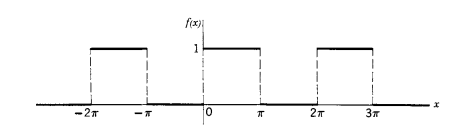
\includegraphics[width=0.7\textwidth]{images/sqwave.png}
        \label{Fig: sqwave}
    \end{center}
    \[
        b_n = \frac{2}{n\pi}(1 - \cos n\pi) =
        \begin{cases} \dfrac{4}{n\pi} & n \text{ odd} \\ 0 & n \text{ even} \end{cases}
    \]
    so
    \[
        f(x) = \frac{4}{\pi}\left(\sin x + \frac{\sin 3x}{3}
               + \frac{\sin 5x}{5} + \cdots \right)
    \]
\end{example}


\subsection{Even and Odd Functions}

\begin{definition}{Even and Odd Functions}{evenodd}
    A function is \emph{even} if $f(-x) = f(x)$ and \emph{odd} if
    $f(-x) = -f(x)$.
\end{definition}
 
Key consequences for Fourier series on $[-L, L]$:
 
\begin{itemize}
    \item \textbf{Even} $f$: all $b_n = 0$; the series contains only cosines.
          \[
              a_n = \frac{2}{L}\int_0^L f(x)\cos\frac{n\pi x}{L}\,dx
          \]
    \item \textbf{Odd} $f$: all $a_n = 0$; the series contains only sines.
          \[
              b_n = \frac{2}{L}\int_0^L f(x)\sin\frac{n\pi x}{L}\,dx
          \]
\end{itemize}
 
Useful identities: even $\times$ even = even; odd $\times$ odd = even;
even $\times$ odd = odd.

\subsection{Half-Range Series}
Given $f(x)$ defined only on $[0, L]$, we can extend it to $[-L, L]$ in
two ways and obtain a \emph{half-range} series:
 
\begin{itemize}
    \item \textbf{Half-range cosine series} (even extension):
          \[
              f(x) = \frac{a_0}{2} + \sum_{n=1}^{\infty}
              a_n\cos\frac{n\pi x}{L}, \qquad
              a_n = \frac{2}{L}\int_0^L f(x)\cos\frac{n\pi x}{L}\,dx
          \]
    \item \textbf{Half-range sine series} (odd extension):
          \[
              f(x) = \sum_{n=1}^{\infty}
              b_n\sin\frac{n\pi x}{L}, \qquad
              b_n = \frac{2}{L}\int_0^L f(x)\sin\frac{n\pi x}{L}\,dx
          \]
\end{itemize}
 
\begin{remark}
    The choice of extension affects convergence at the endpoints $x = 0$
    and $x = L$. The two series are generally different functions outside
    $[0, L]$.
\end{remark}
 

\subsection{Parseval's Theorem}

\begin{theorem}{Parseval's Theorem}{parseval}
    If $f(x)$ has Fourier coefficients $a_n$, $b_n$ on $[-L, L]$, then
    \[
        \frac{1}{L}\int_{-L}^{L} [f(x)]^2\,dx
        = \frac{a_0^2}{2} + \sum_{n=1}^{\infty}(a_n^2 + b_n^2)
    \]
\end{theorem}
 
Parseval's theorem equates the \emph{energy} (mean-square value) of $f$
to the sum of the squared amplitudes of its frequency components. It is
useful for evaluating infinite series.
 
\begin{example}{A classic sum}{parseval-ex}
    The Fourier series of $f(x) = x$ on $[-\pi,\pi]$ gives $b_n = 2(-1)^{n+1}/n$.
    Applying Parseval's theorem:
    \[
        \frac{1}{\pi}\int_{-\pi}^{\pi} x^2\,dx = \sum_{n=1}^{\infty}\frac{4}{n^2}
        \implies \frac{2\pi^2}{3} = 4\sum_{n=1}^{\infty}\frac{1}{n^2}
        \implies \sum_{n=1}^{\infty}\frac{1}{n^2} = \frac{\pi^2}{6}
    \]
\end{example}


\subsection{Fourier Transforms}
 
For a non-periodic function $f(t)$ defined on $(-\infty, \infty)$, the
Fourier series generalizes to the \textbf{Fourier transform pair}:
 
\[
    \hat{f}(\omega) = \int_{-\infty}^{\infty} f(t)\,e^{-i\omega t}\,dt
    \qquad \text{(forward transform)}
\]
\[
    f(t) = \frac{1}{2\pi}\int_{-\infty}^{\infty}
    \hat{f}(\omega)\,e^{i\omega t}\,d\omega
    \qquad \text{(inverse transform)}
\]
 
\subsubsection*{Key Properties}
 
\begin{center}
\begin{tabular}{ll}
    \toprule
    Property & Statement \\
    \midrule
    Linearity      & $\widehat{af + bg} = a\hat{f} + b\hat{g}$ \\[4pt]
    Time shift     & $\widehat{f(t-t_0)} = e^{-i\omega t_0}\hat{f}(\omega)$ \\[4pt]
    Frequency shift & $\widehat{e^{i\omega_0 t}f(t)} = \hat{f}(\omega - \omega_0)$ \\[4pt]
    Differentiation & $\widehat{f'(t)} = i\omega\,\hat{f}(\omega)$ \\[4pt]
    Scaling        & $\widehat{f(at)} = \tfrac{1}{|a|}\hat{f}(\omega/a)$ \\
    \bottomrule
\end{tabular}
\end{center}
 
\subsubsection*{Common Transform Pairs}
 
\[
    e^{-a|t|} \;\longleftrightarrow\; \frac{2a}{a^2 + \omega^2}, \qquad a > 0
\]
\[
    e^{-at^2} \;\longleftrightarrow\; \sqrt{\frac{\pi}{a}}\,e^{-\omega^2/(4a)},
    \qquad a > 0
\]
\[
    \delta(t) \;\longleftrightarrow\; 1, \qquad
    1 \;\longleftrightarrow\; 2\pi\,\delta(\omega)
\]
 
\begin{remark}
    Different textbooks use different conventions for the factor of $2\pi$
    and the sign in the exponent. Boas uses the convention above.
\end{remark}

\subsection{Convolution}
 
\begin{definition}{Convolution}{conv}
    The \emph{convolution} of two functions $f$ and $g$ is
    \[
        (f * g)(t) = \int_{-\infty}^{\infty} f(\tau)\,g(t - \tau)\,d\tau
    \]
\end{definition}
 
\begin{theorem}{Convolution Theorem}{convthm}
    The Fourier transform of a convolution is the product of the transforms:
    \[
        \widehat{f * g}(\omega) = \hat{f}(\omega)\cdot\hat{g}(\omega)
    \]
    Equivalently, the transform of a product is (up to $2\pi$) the
    convolution of the transforms:
    \[
        \widehat{f \cdot g}(\omega)
        = \frac{1}{2\pi}\bigl(\hat{f} * \hat{g}\bigr)(\omega)
    \]
\end{theorem}
 
\subsubsection*{Properties of Convolution}
\begin{itemize}
    \item Commutative: $f * g = g * f$
    \item Associative: $f * (g * h) = (f * g) * h$
    \item Distributive: $f * (g + h) = f*g + f*h$
\end{itemize}
 
\begin{remark}
    Convolution appears naturally in linear systems: if $h(t)$ is the
    impulse response of a system and $x(t)$ is the input, the output is
    $y(t) = (h * x)(t)$.
\end{remark}

\begin{remark}
    I will add given examples from the Final Review here after I am 
    finished going through the chapters.
\end{remark}


\newpage
% ============================================================
% ============================================================
\section{Ordinary Differential Equations}      % Ch. 8
% ============================================================
\begin{abstract}
    \textit{Differential equations} are equations containing derivatives.
    These appear in a great many applied problems involving rates. 
\end{abstract}
\begin{example}{RCL}{RCL}
    Consider a simple series circuit containing a resistane $R$, a capacitance $C$, and inductance $L$, and a source of emf $V$.
    If the current is $I(t)$ and the charge on the capacitor is $q(t)$, then $I = dq/dt$.
    \[
    L\frac{dI}{dt} + RI + \frac{q}{C} = V
    \]
    \[
    L\frac{d^{2}I}{dt^2} + R\frac{dI}{dt} + \frac{I}{C} = \frac{dV}{dt}
    \]
    \begin{minipage}{\linewidth}
        \centering
        \includegraphics[width=0.6\textwidth]{images/rcl.png}
         \label{Fig: rcl}
    \end{minipage}
\end{example}

\subsection{First-Order ODEs}

A first-order ODE has the form $F(x, y, y') = 0$. The main solution methods are:

\subsubsection*{Separable Equations}
If $\dv{y}{x} = f(x)g(y)$, separate and integrate:
\[
    \int \frac{dy}{g(y)} = \int f(x)\,dx
\]

\subsubsection*{Linear Equations}
Standard form: $\dv{y}{x} + P(x)y = Q(x)$. Multiply by the integrating factor
$\mu(x) = e^{\int P(x)\,dx}$:
\[
    \dv{}{x}\bigl[\mu(x)\,y\bigr] = \mu(x)Q(x)
    \implies y = \frac{1}{\mu(x)}\int \mu(x)Q(x)\,dx
\]

\subsubsection*{Exact Equations}
$M(x,y)\,dx + N(x,y)\,dy = 0$ is exact if $\pdv{M}{y} = \pdv{N}{x}$.
Solution: find $F(x,y)$ such that $\pdv{F}{x} = M$ and $\pdv{F}{y} = N$;
then $F(x,y) = C$.


\subsection{Second-Order Linear ODEs}

Standard form: $y'' + P(x)y' + Q(x)y = R(x)$.

\subsubsection*{Homogeneous with Constant Coefficients}
A \textit{Homogeneous Equation} of $x$ and $y$ of degree $n$ means a function
 which can be written as $x^nf(y/x)$ 
For $ay'' + by' + cy = 0$, try $y = e^{rx}$. The characteristic equation is:
\[
    ar^2 + br + c = 0
\]
\begin{center}
\begin{tabular}{ll}
    \toprule
    Roots & General Solution \\
    \midrule
    Two real roots $r_1 \neq r_2$ & $y = c_1 e^{r_1 x} + c_2 e^{r_2 x}$ \\[4pt]
    Repeated root $r_1 = r_2 = r$ & $y = (c_1 + c_2 x)e^{rx}$ \\[4pt]
    Complex roots $r = \alpha \pm i\beta$ & $y = e^{\alpha x}(c_1\cos\beta x + c_2\sin\beta x)$ \\
    \bottomrule
\end{tabular}
\end{center}

\subsubsection*{Method of Undetermined Coefficients}
For $ay'' + by' + cy = R(x)$ where $R(x)$ is a polynomial, exponential,
sine, or cosine — guess a particular solution $y_p$ of the same form as $R(x)$
and solve for coefficients. The general solution is $y = y_h + y_p$.

\begin{remark}
    If $R(x)$ is a solution to the homogeneous equation, multiply your
    guess by $x$ (or $x^2$ if needed) to avoid duplication.
\end{remark}


\subsection{Variation of Parameters}

Given the homogeneous solutions $y_1, y_2$, the particular solution is:
\[
    y_p = -y_1 \int \frac{y_2 R}{W}\,dx + y_2 \int \frac{y_1 R}{W}\,dx
\]
where $W = y_1 y_2' - y_2 y_1'$ is the \textbf{Wronskian}. Works for any $R(x)$,
unlike undetermined coefficients.


\subsection{Power Series Solutions}

For ODEs with non-constant coefficients, assume a solution of the form:
\[
    y = \sum_{n=0}^{\infty} a_n x^n
\]
Substitute into the ODE and match coefficients of each power of $x$ to find
a recurrence relation for $a_n$.

\begin{remark}
    This method works when $x = 0$ is an \emph{ordinary point} — i.e.,
    $P(x)$ and $Q(x)$ are analytic there.
\end{remark}

\begin{example}{Hermite's Equation}{hermite}
    $y'' - 2xy' + 2ny = 0$ has polynomial solutions (Hermite polynomials)
    when $n$ is a non-negative integer, found via the power series method.
\end{example}


\subsection{Frobenius Method}

Used when $x = 0$ is a \textbf{regular singular point} — i.e., $xP(x)$
and $x^2Q(x)$ are analytic at $x = 0$.

Assume a solution of the form:
\[
    y = x^r \sum_{n=0}^{\infty} a_n x^n = \sum_{n=0}^{\infty} a_n x^{n+r},
    \qquad a_0 \neq 0
\]

Substituting gives the \textbf{indicial equation} for $r$:
\[
    r(r-1) + p_0 r + q_0 = 0
\]
where $p_0 = \lim_{x\to 0} xP(x)$ and $q_0 = \lim_{x\to 0} x^2Q(x)$.

\subsubsection*{Cases for Roots $r_1 \geq r_2$}
\begin{itemize}
    \item $r_1 - r_2 \notin \mathbb{Z}$: two independent Frobenius series
    \item $r_1 = r_2$: second solution contains a $\ln x$ term
    \item $r_1 - r_2 \in \mathbb{Z}^+$: second solution may contain a $\ln x$ term
\end{itemize}


\subsection{Bessel's Equation (intro)}

Bessel's equation of order $\nu$ is:
\[
    x^2 y'' + xy' + (x^2 - \nu^2)y = 0
\]
It arises naturally in problems with cylindrical symmetry (e.g.\ heat flow
in a cylinder, vibrating circular membrane).

\subsubsection*{Solutions}
Applying the Frobenius method gives the \textbf{Bessel functions of the first kind}:
\[
    J_\nu(x) = \sum_{n=0}^{\infty}
    \frac{(-1)^n}{n!\,\Gamma(n+\nu+1)}\left(\frac{x}{2}\right)^{2n+\nu}
\]
For non-integer $\nu$, the general solution is $y = AJ_\nu(x) + BJ_{-\nu}(x)$.
For integer $\nu = m$, $J_{-m}$ is not independent; a second solution
$Y_m(x)$ (Bessel function of the second kind) is needed.

\begin{remark}
    Bessel functions are covered in full detail in Chapter 12.
\end{remark}

\subsection{Laplace Transform}

The \textbf{Laplace transform} converts a function of time $f(t)$ into a
function of complex frequency $s$, turning ODEs into algebraic equations.

\begin{definition}{Laplace Transform}{laplace}
    \[
        \mathcal{L}\{f(t)\} = F(s) = \int_0^{\infty} f(t)\,e^{-st}\,dt
    \]
    defined for values of $s$ where the integral converges.
\end{definition}

\subsubsection*{Common Transform Pairs}

\begin{center}
\begin{tabular}{ll}
    \toprule
    $f(t)$ & $F(s) = \mathcal{L}\{f(t)\}$ \\
    \midrule
    $1$                  & $\dfrac{1}{s}$ \\[8pt]
    $t^n$                & $\dfrac{n!}{s^{n+1}}$ \\[8pt]
    $e^{at}$             & $\dfrac{1}{s-a}$ \\[8pt]
    $\sin(\omega t)$     & $\dfrac{\omega}{s^2+\omega^2}$ \\[8pt]
    $\cos(\omega t)$     & $\dfrac{s}{s^2+\omega^2}$ \\[8pt]
    $t^n e^{at}$         & $\dfrac{n!}{(s-a)^{n+1}}$ \\[8pt]
    $\delta(t - a)$      & $e^{-as}$ \\
    \bottomrule
\end{tabular}
\end{center}

\subsubsection*{Key Properties}

\begin{center}
\begin{tabular}{ll}
    \toprule
    Property & Statement \\
    \midrule
    Linearity       & $\mathcal{L}\{af + bg\} = aF(s) + bG(s)$ \\[4pt]
    First derivative & $\mathcal{L}\{f'\} = sF(s) - f(0)$ \\[4pt]
    Second derivative & $\mathcal{L}\{f''\} = s^2F(s) - sf(0) - f'(0)$ \\[4pt]
    $s$-shift        & $\mathcal{L}\{e^{at}f(t)\} = F(s-a)$ \\[4pt]
    $t$-shift        & $\mathcal{L}\{f(t-a)u(t-a)\} = e^{-as}F(s)$ \\[4pt]
    Convolution      & $\mathcal{L}\{f*g\} = F(s)G(s)$ \\
    \bottomrule
\end{tabular}
\end{center}

\subsubsection*{Solving ODEs with the Laplace Transform}

The standard method is:
\begin{enumerate}[(1)]
    \item Take $\mathcal{L}$ of both sides, applying initial conditions
    \item Solve algebraically for $F(s)$
    \item Apply the inverse transform $f(t) = \mathcal{L}^{-1}\{F(s)\}$,
          using partial fractions if needed
\end{enumerate}

\begin{example}{Damped oscillator}{laplace-ex}
    Solve $y'' + 3y' + 2y = e^{-t}$, $y(0) = 0$, $y'(0) = 1$.
    Taking the Laplace transform:
    \[
        s^2Y - 1 + 3sY + 2Y = \frac{1}{s+1}
    \]
    \[
        Y(s) = \frac{1}{(s+1)(s^2+3s+2)} + \frac{1}{s^2+3s+2}
             = \frac{1}{(s+1)^2(s+2)} + \frac{1}{(s+1)(s+2)}
    \]
    Applying partial fractions and inverting gives $y(t)$.
\end{example}

\begin{remark}
    The Laplace transform is particularly powerful for ODEs with
    discontinuous or impulsive forcing, since it handles initial conditions
    automatically.
\end{remark}


\subsection{Dirac Delta}

\begin{definition}{Dirac Delta Function}{dirac}
    The \emph{Dirac delta} $\delta(t - a)$ is not a function in the classical
    sense but a \emph{distribution} defined by:
    \[
        \delta(t - a) = 0 \quad \text{for } t \neq a, \qquad
        \int_{-\infty}^{\infty} \delta(t-a)\,dt = 1
    \]
\end{definition}

\subsubsection*{Sifting Property}

The most important property of the delta function:
\[
    \int_{-\infty}^{\infty} f(t)\,\delta(t - a)\,dt = f(a)
\]
It ``picks out'' the value of $f$ at $t = a$.

\subsubsection*{Useful Identities}
\begin{itemize}
    \item $\delta(t) = \delta(-t)$ \quad (even function)
    \item $\delta(at) = \dfrac{1}{|a|}\delta(t)$
    \item $\delta(t-a) = \dv{}{t}\,u(t-a)$ where $u$ is the Heaviside step function
    \item $f(t)\,\delta(t-a) = f(a)\,\delta(t-a)$
\end{itemize}

\subsubsection*{Laplace Transform}
\[
    \mathcal{L}\{\delta(t-a)\} = e^{-as}, \qquad a \geq 0
\]
In particular, $\mathcal{L}\{\delta(t)\} = 1$.

\begin{example}{Impulse forcing}{delta-ex}
    Consider a mass-spring system struck by an impulse at $t = t_0$:
    \[
        y'' + \omega^2 y = \delta(t - t_0), \qquad y(0) = y'(0) = 0
    \]
    Taking the Laplace transform and inverting:
    \[
        y(t) = \frac{1}{\omega}\sin\bigl(\omega(t - t_0)\bigr)\,u(t - t_0)
    \]
    The system is at rest until $t = t_0$, then oscillates freely.
\end{example}

\begin{remark}
    The delta function can be thought of as the limit of a narrow, tall
    rectangle of unit area as the width shrinks to zero. It models
    instantaneous impulses (forces, charges, heat sources).
\end{remark}


\newpage
% ============================================================
\section{Tensor Analysis}                      % Ch. 10
% ============================================================

\subsection{Cartesian Tensors; Transformation Law}

Under a rotation of coordinate axes, the new coordinates are related to
the old by $x_i' = \sum_j a_{ij} x_j$, where $a_{ij} = \cos\theta_{ij}$
are the direction cosines. The matrix $A = (a_{ij})$ is orthogonal:
\[
    AA^T = A^TA = I \implies \sum_k a_{ik}a_{jk} = \delta_{ij}
\]

\begin{definition}{Cartesian Tensor}{tensor}
    A \emph{tensor of rank $n$} is a quantity with $3^n$ components that
    transform under rotation as:
    \begin{itemize}
        \item \textbf{Rank 0} (scalar): $T' = T$
        \item \textbf{Rank 1} (vector): $T_i' = \sum_j a_{ij} T_j$
        \item \textbf{Rank 2}: $T_{ij}' = \sum_{k,l} a_{ik}\,a_{jl}\,T_{kl}$
        \item \textbf{Rank $n$}: $T_{i_1\cdots i_n}' =
              \sum_{j_1\cdots j_n} a_{i_1 j_1}\cdots a_{i_n j_n}\,T_{j_1\cdots j_n}$
    \end{itemize}
\end{definition}

\begin{remark}
    The transformation law is the defining property of a tensor —
    not just that it has multiple indices, but that its components
    transform in the correct way under rotations.
\end{remark}


\subsection{Tensor Notation and Operations}

\subsubsection*{Einstein Summation Convention}
A repeated index implies summation over that index:
\[
    A_i B_i \equiv \sum_{i=1}^{3} A_i B_i, \qquad
    T_{ij}x_j \equiv \sum_{j=1}^{3} T_{ij}x_j
\]
A \emph{free index} appears once; a \emph{dummy index} appears twice (summed).

\subsubsection*{Basic Operations}
\begin{itemize}
    \item \textbf{Addition:} $S_{ij} + T_{ij}$ — same rank tensors only
    \item \textbf{Outer product:} $T_{ij} = A_i B_j$ — raises rank by combination
    \item \textbf{Contraction:} set two indices equal and sum, e.g.\
          $T_{ii} = \sum_i T_{ii}$ — lowers rank by 2
    \item \textbf{Inner product:} outer product followed by contraction,
          e.g.\ $A_i B_i$ (dot product), $T_{ij}S_{jk}$ (matrix multiply)
\end{itemize}

\subsubsection*{Symmetric and Antisymmetric Parts}
Any rank-2 tensor can be decomposed as:
\[
    T_{ij} = \underbrace{\frac{1}{2}(T_{ij} + T_{ji})}_{\text{symmetric } S_{ij}}
           + \underbrace{\frac{1}{2}(T_{ij} - T_{ji})}_{\text{antisymmetric } A_{ij}}
\]
Note that $S_{ij}A_{ij} = 0$ always.


\subsection{Inertia Tensor}

The inertia tensor is a physical rank-2 tensor relating angular momentum
$\vv{L}$ to angular velocity $\vv{\omega}$:
\[
    L_i = \sum_j I_{ij}\,\omega_j, \qquad \text{i.e.,} \quad \vv{L} = I\,\vv{\omega}
\]
For a collection of mass points:
\[
    I_{ij} = \sum_\alpha m_\alpha
    \bigl(\delta_{ij}|\vv{r}_\alpha|^2 - x_{\alpha i}\,x_{\alpha j}\bigr)
\]
Written out, the diagonal elements are the familiar moments of inertia
(e.g.\ $I_{xx} = \sum m(y^2 + z^2)$) and the off-diagonal elements are
the products of inertia (e.g.\ $I_{xy} = -\sum m\,xy$).

\begin{remark}
    Since $I_{ij}$ is real and symmetric, it can always be diagonalized
    by rotating to the \emph{principal axes}, where $\vv{L} = I\vv{\omega}$
    with $I$ diagonal.
\end{remark}


\subsection{Kronecker Delta and Levi-Civita Symbol}

\subsubsection*{Kronecker Delta}
\[
    \delta_{ij} = \begin{cases} 1 & i = j \\ 0 & i \neq j \end{cases}
\]
It is an isotropic rank-2 tensor: same components in every frame.
Key identity: $\delta_{ij}x_j = x_i$, \quad $\delta_{ii} = 3$.

\subsubsection*{Levi-Civita Symbol}
\[
    \varepsilon_{ijk} = \begin{cases}
        +1 & \text{if } (i,j,k) \text{ is an even permutation of } (1,2,3) \\
        -1 & \text{if } (i,j,k) \text{ is an odd permutation of } (1,2,3) \\
        0  & \text{if any two indices are equal}
    \end{cases}
\]

Used to write the cross product and curl compactly:
\[
    (\vv{A}\times\vv{B})_i = \varepsilon_{ijk}A_j B_k, \qquad
    (\curl\vv{A})_i = \varepsilon_{ijk}\pdv{A_k}{x_j}
\]

\subsubsection*{Key Identity}
\[
    \varepsilon_{ijk}\,\varepsilon_{ilm} = \delta_{jl}\delta_{km} - \delta_{jm}\delta_{kl}
\]
This is used to prove vector identities such as
$\vv{A}\times(\vv{B}\times\vv{C}) = \vv{B}(\vv{A}\cdot\vv{C})
- \vv{C}(\vv{A}\cdot\vv{B})$.


\subsection{Pseudovectors and Pseudotensors}

\begin{definition}{Pseudotensor}{pseudo}
    A \emph{pseudotensor} transforms like a tensor under proper rotations
    (det $A = +1$) but picks up an extra sign flip under improper rotations
    (reflections, det $A = -1$):
    \[
        T_{ij\cdots}' = (\det A)\sum a_{ik}a_{jl}\cdots T_{kl\cdots}
    \]
    A \emph{pseudovector} (axial vector) is a rank-1 pseudotensor.
\end{definition}

Common pseudovectors: angular momentum $\vv{L} = \vv{r}\times\vv{p}$,
magnetic field $\vv{B}$, torque $\vv{\tau}$. Common polar (true) vectors:
position $\vv{r}$, force $\vv{F}$, electric field $\vv{E}$.

\begin{remark}
    The cross product of two polar vectors is a pseudovector.
    The Levi-Civita symbol $\varepsilon_{ijk}$ is itself a pseudotensor.
\end{remark}


\subsection{More About Applications}

Tensors appear throughout physics wherever a linear relationship exists
between vector quantities:

\begin{itemize}
    \item \textbf{Stress tensor} $\sigma_{ij}$: force per unit area on a surface;
          $F_i = \sigma_{ij}n_j$
    \item \textbf{Strain tensor} $e_{ij}$: deformation of a solid;
          symmetric, related to stress by Hooke's law $\sigma_{ij} = C_{ijkl}e_{kl}$
    \item \textbf{Polarizability tensor} $\alpha_{ij}$: relates induced dipole
          to applied field, $p_i = \alpha_{ij}E_j$
    \item \textbf{Conductivity tensor} $\sigma_{ij}$: $J_i = \sigma_{ij}E_j$
          in anisotropic media
\end{itemize}


\subsection{Curvilinear Coordinates}

For non-Cartesian coordinate systems $(q_1, q_2, q_3)$, position is given
by $\vv{r} = \vv{r}(q_1, q_2, q_3)$. The \textbf{scale factors} are:
\[
    h_i = \left|\pdv{\vv{r}}{q_i}\right|
\]
A coordinate system is \emph{orthogonal} if $\pdv{\vv{r}}{q_i}\cdot\pdv{\vv{r}}{q_j} = 0$
for $i\neq j$. The arc length element is:
\[
    ds^2 = h_1^2\,dq_1^2 + h_2^2\,dq_2^2 + h_3^2\,dq_3^2
\]

\begin{center}
\begin{tabular}{lccc}
    \toprule
    System & $q_1, q_2, q_3$ & $h_1, h_2, h_3$ & Volume element \\
    \midrule
    Cartesian   & $x,y,z$          & $1,1,1$          & $dx\,dy\,dz$ \\[4pt]
    Cylindrical & $r,\phi,z$       & $1,r,1$          & $r\,dr\,d\phi\,dz$ \\[4pt]
    Spherical   & $r,\theta,\phi$  & $1,r,r\sin\theta$& $r^2\sin\theta\,dr\,d\theta\,d\phi$ \\
    \bottomrule
\end{tabular}
\end{center}


\subsection{Vector Operators in Orthogonal Curvilinear Coordinates}

In orthogonal curvilinear coordinates with scale factors $h_1, h_2, h_3$:

\subsubsection*{Gradient}
\[
    \grad f = \frac{1}{h_1}\pdv{f}{q_1}\,\hat{e}_1
            + \frac{1}{h_2}\pdv{f}{q_2}\,\hat{e}_2
            + \frac{1}{h_3}\pdv{f}{q_3}\,\hat{e}_3
\]

\subsubsection*{Divergence}
\[
    \div\vv{A} = \frac{1}{h_1 h_2 h_3}\left[
        \pdv{}{q_1}(h_2 h_3 A_1) +
        \pdv{}{q_2}(h_1 h_3 A_2) +
        \pdv{}{q_3}(h_1 h_2 A_3)
    \right]
\]

\subsubsection*{Laplacian}
\[
    \nabla^2 f = \frac{1}{h_1 h_2 h_3}\left[
        \pdv{}{q_1}\!\left(\frac{h_2 h_3}{h_1}\pdv{f}{q_1}\right) +
        \pdv{}{q_2}\!\left(\frac{h_1 h_3}{h_2}\pdv{f}{q_2}\right) +
        \pdv{}{q_3}\!\left(\frac{h_1 h_2}{h_3}\pdv{f}{q_3}\right)
    \right]
\]

\begin{example}{Laplacian in Spherical Coordinates}{laplacian-sph}
    With $h_1 = 1$, $h_2 = r$, $h_3 = r\sin\theta$:
    \[
        \nabla^2 f = \frac{1}{r^2}\pdv{}{r}\!\left(r^2\pdv{f}{r}\right)
                   + \frac{1}{r^2\sin\theta}\pdv{}{\theta}\!\left(\sin\theta\pdv{f}{\theta}\right)
                   + \frac{1}{r^2\sin^2\theta}\pdv[2]{f}{\phi}
    \]
\end{example}


\subsection{Non-Cartesian Tensors}

In general curvilinear coordinates, tensors must account for the fact that
basis vectors change from point to point. This requires distinguishing
between \emph{covariant} and \emph{contravariant} components.

\begin{definition}{Covariant and Contravariant}{cocon}
    For a coordinate transformation $x^i \to x^{i'}$:
    \begin{itemize}
        \item \textbf{Contravariant} components transform as:
              $V^{i'} = \sum_j \pdv{x^{i'}}{x^j} V^j$
        \item \textbf{Covariant} components transform as:
              $V_{i'} = \sum_j \pdv{x^j}{x^{i'}} V_j$
    \end{itemize}
\end{definition}

The \textbf{metric tensor} $g_{ij}$ encodes the geometry of the space:
\[
    ds^2 = g_{ij}\,dx^i\,dx^j, \qquad
    g_{ij} = \pdv{\vv{r}}{x^i}\cdot\pdv{\vv{r}}{x^j}
\]
It is used to raise and lower indices: $V_i = g_{ij}V^j$.

\begin{remark}
    For orthogonal curvilinear coordinates, $g_{ij} = h_i^2\,\delta_{ij}$
    (no off-diagonal terms), recovering the scale factor formulas above.
    In Cartesian coordinates $g_{ij} = \delta_{ij}$, so covariant and
    contravariant components are identical.
\end{remark}




\newpage
% ============================================================
\section{Series Solutions and Special Functions} % Ch. 12 (no spherical harmonics)
% ============================================================

\subsection{Legendre's Equation}

\subsection{Leibniz' Rule for Differentiating Products}

\subsection{Legendre Polynomials}



\subsection{Orthogonality and Expansion}

\subsection{Normalizat6ion of the Legendre Polynomials}

\subsection{Legendre Series}
\subsection{Associated Legendr Functiohs}

\subsection{Bessel's Equation}



\subsection{Bessel Functions \(J_\nu\) and \(Y_\nu\)}



\subsection{Orthogonality of Bessel Functions}



\subsection{Applications}



\newpage
% ============================================================
\section{Partial Differential Equations}        % Ch. 13
% ============================================================

\subsection{Separation of Variables}

The central technique for solving linear PDEs on bounded domains.
Assume the solution factors as a product of single-variable functions,
e.g.\ $u(x,t) = X(x)T(t)$, substitute into the PDE, and divide through
to separate the variables:
\[
    \frac{1}{T}\dv{T}{t} = \frac{1}{X}\dv[2]{X}{x} = -\lambda
\]
Each side depends on a different variable, so both must equal the same
constant $-\lambda$ (the \textbf{separation constant}). This yields two ODEs
which are solved subject to the boundary and initial conditions.

\begin{remark}
    The sign and value of $\lambda$ is determined by the boundary conditions.
    For most physical problems with homogeneous BCs, $\lambda > 0$ gives
    oscillatory spatial solutions.
\end{remark}


\subsection{Heat Equation}

Models diffusion of heat (or any scalar quantity) in a medium:
\[
    \pdv{u}{t} = \kappa\,\nabla^2 u
\]
where $\kappa > 0$ is the thermal diffusivity.

\subsubsection*{1D Heat Equation on $[0,L]$}
With boundary conditions $u(0,t) = u(L,t) = 0$ and initial condition
$u(x,0) = f(x)$, separation of variables gives $u = X(x)T(t)$:
\[
    T' + \kappa\lambda T = 0, \qquad X'' + \lambda X = 0
\]
The BCs force $\lambda_n = (n\pi/L)^2$ and $X_n = \sin(n\pi x/L)$.
The general solution is:
\[
    u(x,t) = \sum_{n=1}^{\infty} b_n \sin\frac{n\pi x}{L}\,
              e^{-\kappa(n\pi/L)^2 t}
\]
where $b_n = \dfrac{2}{L}\displaystyle\int_0^L f(x)\sin\dfrac{n\pi x}{L}\,dx$.

\begin{remark}
    The exponential decay $e^{-\kappa\lambda_n t}$ means higher harmonics
    decay faster. As $t\to\infty$, $u\to 0$ (heat flows out through the ends).
    For insulated ends ($u_x = 0$ at $x=0,L$), eigenfunctions become cosines
    and $u\to$ the average of $f$.
\end{remark}


\subsection{Wave Equation}

Models vibrations of strings, membranes, sound, and electromagnetic waves:
\[
    \pdv[2]{u}{t} = c^2\,\nabla^2 u
\]
where $c$ is the wave speed.

\subsubsection*{1D Wave Equation on $[0,L]$}
With $u(0,t) = u(L,t) = 0$, $u(x,0) = f(x)$, $u_t(x,0) = g(x)$:
\[
    u(x,t) = \sum_{n=1}^{\infty} \sin\frac{n\pi x}{L}
    \left(A_n\cos\frac{n\pi ct}{L} + B_n\sin\frac{n\pi ct}{L}\right)
\]
\[
    A_n = \frac{2}{L}\int_0^L f(x)\sin\frac{n\pi x}{L}\,dx, \qquad
    B_n = \frac{2}{n\pi c}\int_0^L g(x)\sin\frac{n\pi x}{L}\,dx
\]

\subsubsection*{D'Alembert's Solution}
For the infinite string $(-\infty < x < \infty)$:
\[
    u(x,t) = \frac{1}{2}\bigl[f(x+ct) + f(x-ct)\bigr]
            + \frac{1}{2c}\int_{x-ct}^{x+ct} g(s)\,ds
\]
This shows the solution as two waves traveling in opposite directions.


\subsection{Laplace's Equation}

Describes steady-state (time-independent) phenomena — electrostatics,
gravitational potential, steady-state temperature:
\[
    \nabla^2 u = 0
\]
Solutions are called \textbf{harmonic functions}.

\subsubsection*{2D Cartesian: Rectangle}
On $0\leq x\leq a$, $0\leq y\leq b$ with $u=0$ on three sides and
$u(x,b) = f(x)$:
\[
    u(x,y) = \sum_{n=1}^{\infty} C_n \sin\frac{n\pi x}{a}
              \sinh\frac{n\pi y}{a}, \qquad
    C_n = \frac{2}{a\sinh(n\pi b/a)}\int_0^a f(x)\sin\frac{n\pi x}{a}\,dx
\]

\subsubsection*{2D Polar: Disk}
On a disk of radius $a$ with $u(a,\phi) = f(\phi)$:
\[
    u(r,\phi) = \frac{a_0}{2} + \sum_{n=1}^{\infty}
    \left(\frac{r}{a}\right)^n (a_n\cos n\phi + b_n\sin n\phi)
\]
where $a_n$, $b_n$ are the Fourier coefficients of $f(\phi)$.

\begin{remark}
    \textbf{Mean value theorem for harmonic functions:} the value of $u$
    at the center of any circle equals the average of $u$ on the circle.
\end{remark}


\subsection{Poisson's Equation}

The inhomogeneous version of Laplace's equation with a source term:
\[
    \nabla^2 u = \rho(x,y,z)
\]
where $\rho$ represents a source density (charge, heat generation, etc.).

\subsubsection*{Solution Strategy}
Write $u = u_h + u_p$ where $\nabla^2 u_h = 0$ (satisfies BCs) and
$u_p$ is any particular solution of $\nabla^2 u_p = \rho$.

\subsubsection*{Green's Function}
The formal solution can be written using a Green's function $G(\vv{r},\vv{r}')$
satisfying $\nabla^2 G = \delta^3(\vv{r}-\vv{r}')$:
\[
    u(\vv{r}) = \int G(\vv{r},\vv{r}')\,\rho(\vv{r}')\,d^3r'
\]
In free space (3D): $G(\vv{r},\vv{r}') = -\dfrac{1}{4\pi|\vv{r}-\vv{r}'|}$.


\subsection{Boundary Conditions}

The three standard types of boundary conditions for PDEs:
\begin{itemize}
    \item \textbf{Dirichlet:} $u$ is specified on the boundary,
          e.g.\ $u\big|_{\partial D} = f$. Models fixed temperature or potential.
    \item \textbf{Neumann:} the normal derivative $\pdv{u}{n}$ is specified
          on the boundary. Models insulated surfaces (heat flux = 0) or
          specified flux.
    \item \textbf{Robin (mixed):} a linear combination
          $\alpha u + \beta\pdv{u}{n} = f$ on the boundary.
          Models Newton's law of cooling.
\end{itemize}

\begin{remark}
    For the heat and wave equations, we also need \textbf{initial conditions}:
    the value of $u$ (and $u_t$ for the wave equation) at $t=0$.
    A well-posed problem requires the right number and type of conditions.
\end{remark}


\subsection{Sturm--Liouville Theory}

Many separation of variables problems produce an eigenvalue equation of the form:
\[
    \dv{}{x}\!\left[p(x)\dv{y}{x}\right] - q(x)y + \lambda w(x)y = 0,
    \qquad x\in[a,b]
\]
with appropriate homogeneous BCs. This is the \textbf{Sturm--Liouville problem}.

\begin{theorem}{Sturm--Liouville}{SL}
    Under suitable conditions on $p, q, w$ (with $p, w > 0$):
    \begin{enumerate}[(i)]
        \item All eigenvalues $\lambda_n$ are real, and $\lambda_1 < \lambda_2 < \cdots \to \infty$
        \item Eigenfunctions $y_n$ corresponding to distinct eigenvalues are
              orthogonal with weight $w(x)$:
              \[
                  \int_a^b y_m(x)\,y_n(x)\,w(x)\,dx = 0, \quad m\neq n
              \]
        \item The eigenfunctions form a complete set: any piecewise smooth
              $f$ can be expanded as $f(x) = \sum_n c_n y_n(x)$
    \end{enumerate}
\end{theorem}

Common Sturm--Liouville problems and their eigenfunctions:
\begin{center}
\begin{tabular}{lll}
    \toprule
    Equation & Eigenfunctions & Weight $w$ \\
    \midrule
    $y'' + \lambda y = 0$ on $[0,L]$ & $\sin(n\pi x/L)$ or $\cos(n\pi x/L)$ & $1$ \\[4pt]
    Legendre's equation on $[-1,1]$  & $P_n(x)$ & $1$ \\[4pt]
    Bessel's equation on $[0,a]$     & $J_\nu(\alpha_{nm} x/a)$ & $x$ \\
    \bottomrule
\end{tabular}
\end{center}


\subsection{2D and 3D Problems}

\subsubsection*{Rectangular Membrane (2D Wave Equation)}
On $0\leq x\leq a$, $0\leq y\leq b$ with $u=0$ on all edges:
\[
    u(x,y,t) = \sum_{m,n} \sin\frac{m\pi x}{a}\sin\frac{n\pi y}{b}
    \left(A_{mn}\cos\omega_{mn}t + B_{mn}\sin\omega_{mn}t\right)
\]
\[
    \omega_{mn} = c\pi\sqrt{\frac{m^2}{a^2} + \frac{n^2}{b^2}}
\]

\subsubsection*{Laplace's Equation in 3D Spherical Coordinates}
Separating $u = R(r)\Theta(\theta)\Phi(\phi)$ gives:
\[
    u(r,\theta,\phi) = \sum_{\ell,m}
    \left(A_{\ell m} r^\ell + B_{\ell m} r^{-\ell-1}\right)
    P_\ell^m(\cos\theta)\,e^{im\phi}
\]
where $P_\ell^m$ are associated Legendre functions. For azimuthal symmetry
($\phi$-independent), only $m=0$ terms survive and $P_\ell^0 = P_\ell$
(ordinary Legendre polynomials).

\subsubsection*{Heat/Wave in a Cylinder}
Separation in cylindrical coordinates $(r,\phi,z)$ leads to Bessel's equation
in $r$, giving solutions $J_n(\alpha r)$ and $Y_n(\alpha r)$. For a solid
cylinder, regularity at $r=0$ requires discarding $Y_n$; the eigenvalues
$\alpha_{nm}$ are determined by the zeros of $J_n$.

\newpage
% ============================================================
\section{Functions of a Complex Variable}       % Ch. 14
% ============================================================

\subsection{Analytic Functions (revisited)}

A function $f(z) = u(x,y) + iv(x,y)$ is \textbf{analytic} at $z_0$ if
$f'(z_0)$ exists in some neighborhood of $z_0$.

\subsubsection*{Cauchy--Riemann Equations}
A necessary condition for analyticity:
\[
    \pdv{u}{x} = \pdv{v}{y}, \qquad \pdv{u}{y} = -\pdv{v}{x}
\]
If $u$ and $v$ have continuous first partial derivatives and satisfy C--R,
then $f$ is analytic. The derivative is then:
\[
    f'(z) = \pdv{u}{x} + i\pdv{v}{x} = \pdv{v}{y} - i\pdv{u}{y}
\]

\begin{remark}
    Both $u$ and $v$ satisfy Laplace's equation $\nabla^2 u = \nabla^2 v = 0$
    whenever $f$ is analytic. They are called \emph{harmonic conjugates}.
\end{remark}


\subsection{Contour Integrals}

For a complex function $f(z)$ along a curve $C$ parameterized by
$z(t) = x(t) + iy(t)$, $t \in [a,b]$:
\[
    \int_C f(z)\,dz = \int_a^b f(z(t))\,z'(t)\,dt
\]

\subsubsection*{ML Inequality}
A useful bound on contour integrals:
\[
    \left|\int_C f(z)\,dz\right| \leq ML
\]
where $M = \max_{z\in C}|f(z)|$ and $L$ is the arc length of $C$.

\begin{example}{A simple contour integral}{contour-ex}
    Evaluate $\int_C \bar{z}\,dz$ along the straight line from $0$ to $1+i$.
    Parameterize: $z(t) = t + it$, $t\in[0,1]$, so $z'(t) = 1+i$ and
    $\bar{z} = t - it$. Then:
    \[
        \int_C \bar{z}\,dz = \int_0^1 (t-it)(1+i)\,dt
        = (1+i)\int_0^1 t(1-i)\,dt = (1+i)(1-i)\cdot\tfrac{1}{2} = 1
    \]
\end{example}


\subsection{Cauchy's Theorem and Integral Formula}

\begin{theorem}{Cauchy's Theorem}{cauchythm}
    If $f(z)$ is analytic everywhere inside and on a simple closed contour $C$,
    then:
    \[
        \oint_C f(z)\,dz = 0
    \]
\end{theorem}

\begin{theorem}{Cauchy's Integral Formula}{cauchyif}
    If $f(z)$ is analytic inside and on $C$, and $z_0$ is any point inside $C$:
    \[
        f(z_0) = \frac{1}{2\pi i}\oint_C \frac{f(z)}{z - z_0}\,dz
    \]
    More generally, for the $n$-th derivative:
    \[
        f^{(n)}(z_0) = \frac{n!}{2\pi i}\oint_C \frac{f(z)}{(z-z_0)^{n+1}}\,dz
    \]
\end{theorem}

\begin{remark}
    Cauchy's integral formula is remarkable: knowing $f$ on the boundary $C$
    completely determines $f$ (and all its derivatives) inside $C$.
\end{remark}


\subsection{Laurent Series}

If $f(z)$ is analytic in an annulus $r < |z - z_0| < R$, it can be expanded as:
\[
    f(z) = \sum_{n=-\infty}^{\infty} c_n (z - z_0)^n
\]
where
\[
    c_n = \frac{1}{2\pi i}\oint_C \frac{f(z)}{(z-z_0)^{n+1}}\,dz
\]
The \textbf{principal part} is the sum of terms with $n < 0$. The coefficient
$c_{-1}$ is the \textbf{residue} of $f$ at $z_0$.

\begin{remark}
    A Taylor series is a Laurent series with no negative powers — valid only
    when $f$ is analytic at $z_0$ itself.
\end{remark}


\subsection{Singularities and Residues}

\begin{definition}{Types of Singularities}{sing}
    At an isolated singularity $z_0$:
    \begin{itemize}
        \item \textbf{Removable singularity:} principal part vanishes;
              $f$ can be redefined to be analytic at $z_0$
        \item \textbf{Pole of order $m$:} principal part has finitely many
              terms; $c_{-m} \neq 0$ and $c_n = 0$ for $n < -m$
        \item \textbf{Essential singularity:} principal part has infinitely
              many terms (e.g.\ $e^{1/z}$ at $z=0$)
    \end{itemize}
\end{definition}

\subsubsection*{Computing Residues}

For a \textbf{simple pole} ($m=1$) at $z_0$:
\[
    \Res(f, z_0) = \lim_{z \to z_0}(z - z_0)f(z)
\]
For a \textbf{pole of order $m$} at $z_0$:
\[
    \Res(f, z_0) = \frac{1}{(m-1)!}\lim_{z\to z_0}
    \dv[m-1]{}{z}\bigl[(z-z_0)^m f(z)\bigr]
\]
For $f(z) = p(z)/q(z)$ with a simple pole where $q(z_0)=0$, $p(z_0)\neq 0$:
\[
    \Res(f, z_0) = \frac{p(z_0)}{q'(z_0)}
\]


\subsection{Residue Theorem}

\begin{theorem}{Residue Theorem}{residue}
    If $f(z)$ is analytic inside and on a simple closed contour $C$ except
    at isolated singularities $z_1, z_2, \ldots, z_n$ inside $C$:
    \[
        \oint_C f(z)\,dz = 2\pi i \sum_{k=1}^{n} \Res(f, z_k)
    \]
\end{theorem}

\begin{remark}
    The contour $C$ is traversed counterclockwise (positive orientation).
    For clockwise traversal, the result picks up a minus sign.
\end{remark}


\subsection{Evaluation of Real Integrals}

\subsubsection*{Type I: $\int_{-\infty}^{\infty} R(x)\,dx$}
Close the contour with a semicircle in the upper half-plane (UHP).
Jordan's lemma guarantees the semicircle contributes $0$ as $|z|\to\infty$
provided $|f(z)| \to 0$ fast enough. Then:
\[
    \int_{-\infty}^{\infty} R(x)\,dx = 2\pi i \sum_{\Im z_k > 0} \Res(R, z_k)
\]

\subsubsection*{Type II: $\int_0^{2\pi} R(\cos\theta, \sin\theta)\,d\theta$}
Substitute $z = e^{i\theta}$, $d\theta = dz/(iz)$:
\[
    \cos\theta = \frac{z + z^{-1}}{2}, \qquad
    \sin\theta = \frac{z - z^{-1}}{2i}
\]
The integral becomes a contour integral over the unit circle $|z|=1$.

\subsubsection*{Type III: $\int_{-\infty}^{\infty} R(x)e^{i\alpha x}\,dx$}
Use \textbf{Jordan's Lemma}: for $\alpha > 0$, close in the UHP;
for $\alpha < 0$, close in the lower half-plane.
\[
    \int_{-\infty}^{\infty} R(x)e^{i\alpha x}\,dx
    = 2\pi i \sum_{\Im z_k > 0} \Res\bigl(R(z)e^{i\alpha z},\, z_k\bigr)
\]


\subsection{Mapping}

An analytic function $w = f(z)$ defines a \textbf{conformal mapping} from
the $z$-plane to the $w$-plane — it preserves angles between curves at
points where $f'(z) \neq 0$.

\subsubsection*{Common Mappings}
\begin{itemize}
    \item \textbf{Linear:} $w = az + b$ — rotation, scaling, translation
    \item \textbf{Inversion:} $w = 1/z$ — maps circles/lines to circles/lines
    \item \textbf{Joukowski:} $w = z + 1/z$ — maps circles to airfoil shapes
    \item \textbf{Exponential:} $w = e^z$ — maps horizontal strips to sectors
    \item \textbf{Möbius (bilinear):} $w = \dfrac{az+b}{cz+d}$ —
          maps circles/lines to circles/lines
\end{itemize}

\begin{remark}
    A Möbius transformation is determined by specifying where three points map.
    It maps the real axis to itself if $a,b,c,d \in \mathbb{R}$.
\end{remark}


\subsection{Applications of Mapping}

Conformal mapping is used to solve 2D boundary value problems
(Laplace's equation) by transforming a complicated domain into a
simpler one where the solution is known.

\subsubsection*{Method}
\begin{enumerate}[(1)]
    \item Find a conformal map $w = f(z)$ taking the given domain $D$
          to a simpler domain $D'$ (e.g.\ upper half-plane or unit disk)
    \item Solve $\nabla^2 \Phi = 0$ with the transformed boundary conditions in $D'$
    \item Pull the solution back: $\phi(x,y) = \Phi(u(x,y),\, v(x,y))$
\end{enumerate}

\begin{example}{Electrostatics}{mapping-ex}
    To find the electric potential between two non-parallel conducting plates,
    map the wedge-shaped region to the upper half-plane using $w = z^{\pi/\alpha}$
    where $\alpha$ is the opening angle. The potential in the half-plane is
    simply $\Phi = A\arg(w) + B$, which pulls back to $\phi = A\theta + B$
    in polar coordinates — a linear function of angle.
\end{example}

\newpage
% ============================================================
\section{Final Review Notes}       % Ch. 14
% ============================================================
\subsection{A: Linear Algebra and Index Notation}
\subsection{B: Series and Integral Transorms}
\subsubsection{B.1}
ratio test, range of convergence (simple, AP Calc BC)
\subsubsection{B.2}
Parametric form $\vec{r} = \vec{r_0} + \lambda \hat{t}$
where $\vec{r}$ is the line, $\vec{r_0}$ is an initial point on the line,
 $\lambda$ is some scalar factor that shifts you along the line, and $\hat{t}$ 
 is the direction of the line. The equation of a plane is a $\hat{n}$ 
 which tells you the direction the plane faces (use cross product). 
 Plug in any point on that plane to finalize the equation.
 Use $\frac{|ax_1 + by_1 + cz_1 - d|}{\sqrt{a^2 + b^2+ c^2}}$ to solve for shortest distance.
\subsection{B.3}
A function must satisfy the Dirichlet-type conditions: periodicity, single-valuedness
, piecewise continuity with only finitely many discontinuities per period, finite many extrema.
\subsection{B.4}
If a function is odd, the Fourier series only has sine terms.
\[
x = \sum_{n=1}{\infty} b_nsin(nx), b_n= \frac{1}{\pi} \int_{-\pi}^{\pi} xsin(nx)dx
\]
\subsection{C: Vector Calculus, Potentials, Special Functions}

\subsection{D: ODEs and PDEs}
% ============================================================
\appendix
\section{Formula Sheet}
% ============================================================

\subsection*{Legendre Polynomials}



\subsection*{Bessel Function Zeros}



\subsection*{Gamma Function}



\subsection*{Common Fourier Transforms}



\subsection*{Vector Identities}



\end{document}